
% TODO: Name all appendices properly in an incremental order!!

% \vspace{-7mm}
% {\let\clearpage\relax
\chapter{Appendix A - Concept Map}
% }
\label{appendix:A-concept-map}
% concept map

\begin{figure}[h!]
\centering
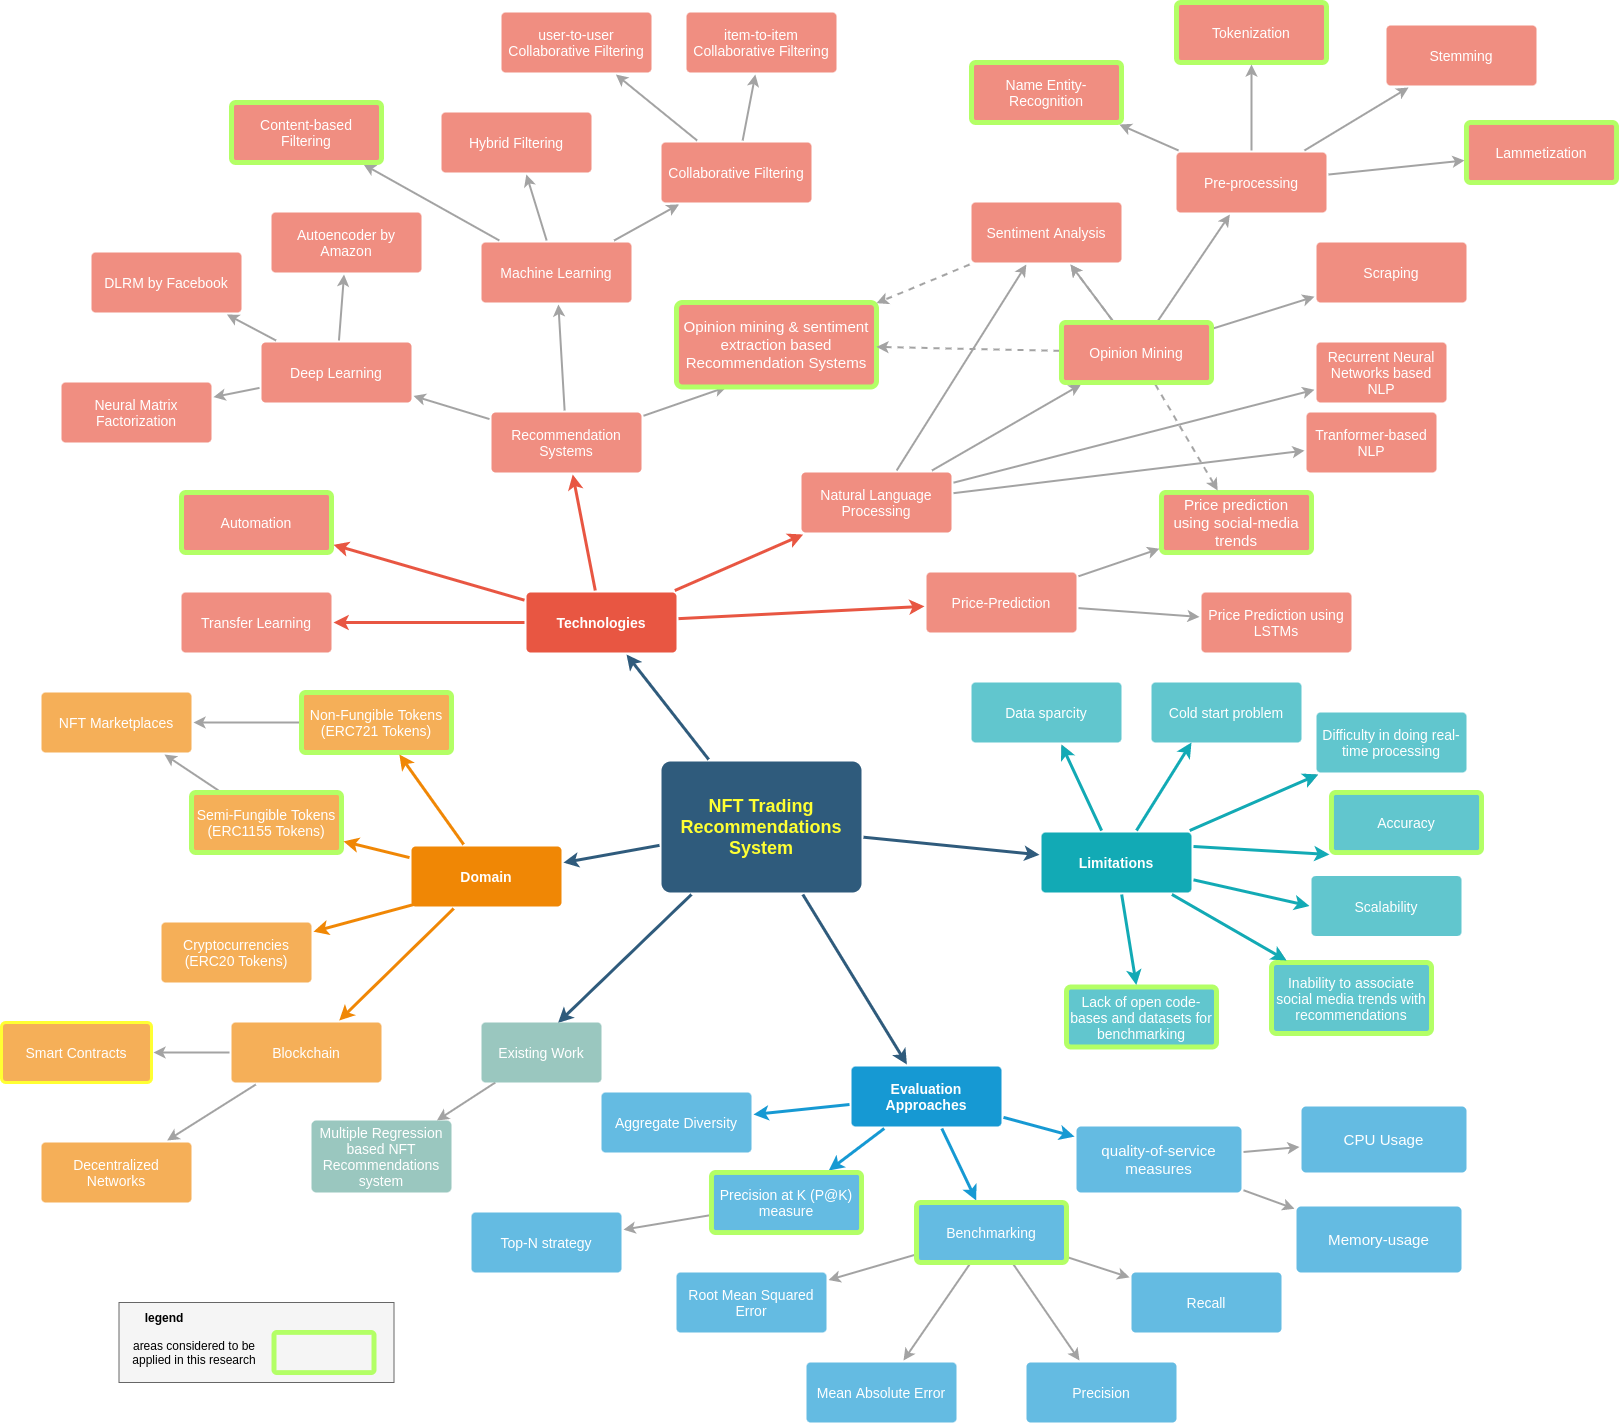
\includegraphics[width=\textwidth]{images/appendix/concept-map.png}
\caption{Concept Map \textit{(self-composed)}}
\label{fig:concept-map}
\end{figure}

\chapter{Appendix B - Gantt Chart}
% }
\label{appendix:B-gantt-chart}

% Gantt Chart
\begin{figure}[h!]
\centering
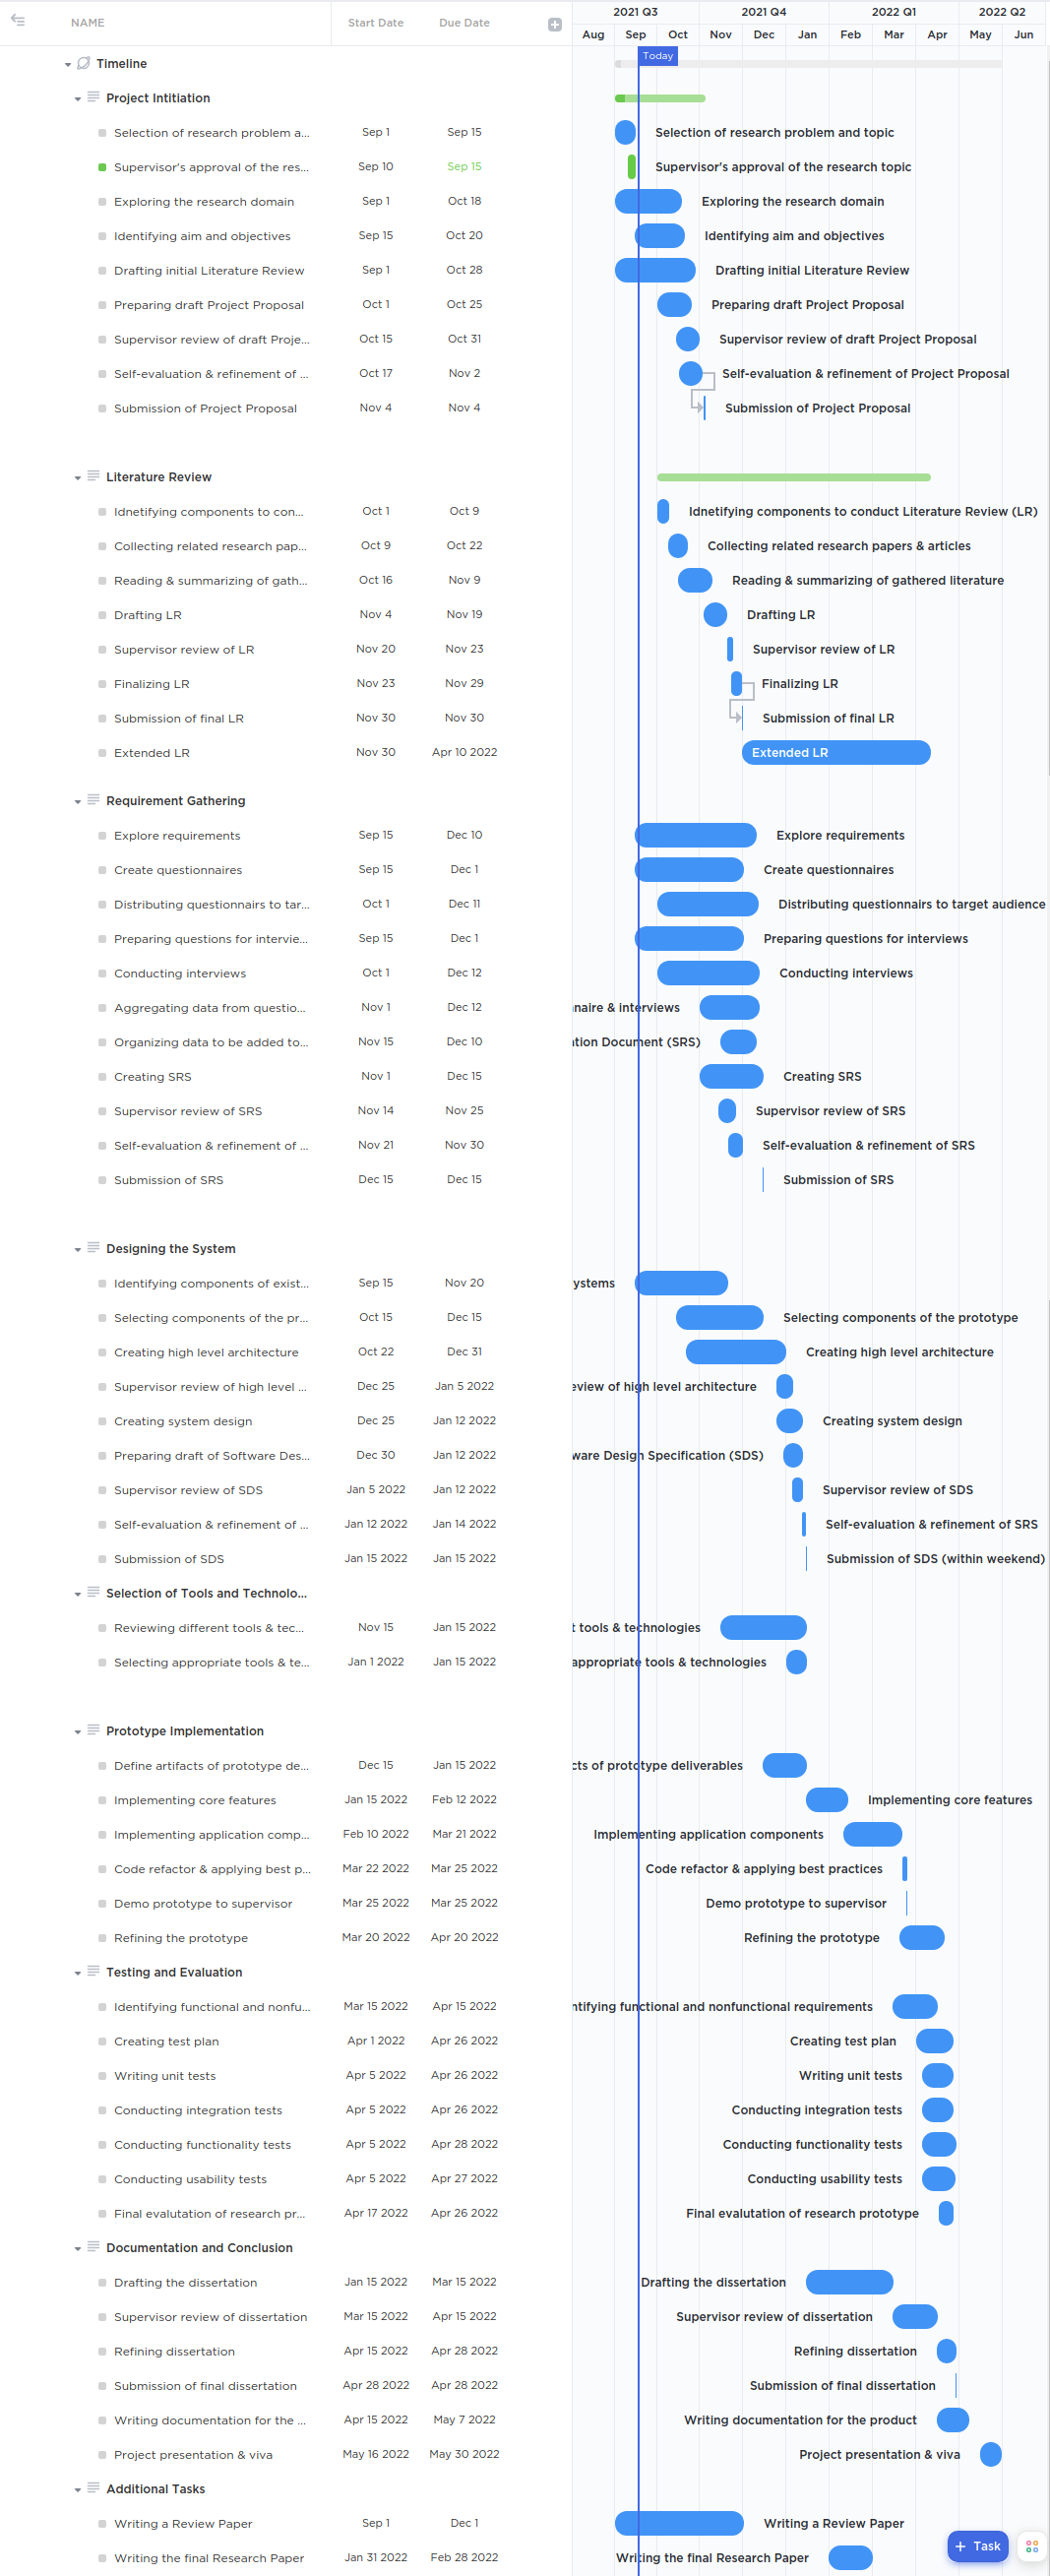
\includegraphics[width=0.8\textwidth,height=0.85\textheight]{images/gantt-chart.png}
\caption{Gantt Chart}
\end{figure}

% \chapter{Appendix B - Work Breakdown Structure}

% \chapter{Appendix  - Requirement Engineering Survey} (questionnaire)


\chapter{Appendix C - Design}
\label{appendix:design}

\begin{figure}[h!]
\centering
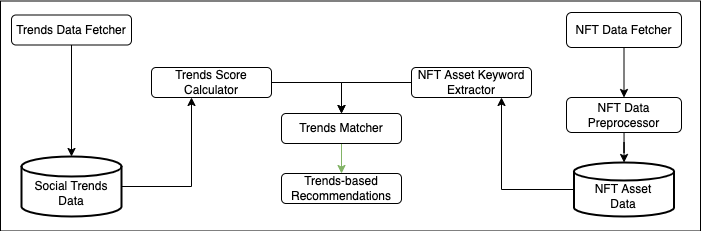
\includegraphics[width=\textwidth]{images/Design/trends-system-process.png}
\caption{Trends based Recommendations Process Flowchart \textit{(self-composed)}}
\label{fig:trends-process-flowchart}
\end{figure}

\chapter{Appendix D - Implementation}
\label{appendix:implementation}

\section*{Appendix D1 - Implementation Code Snippets}

% Tweet Volume Calculation
\begin{figure}[h!]
\centering
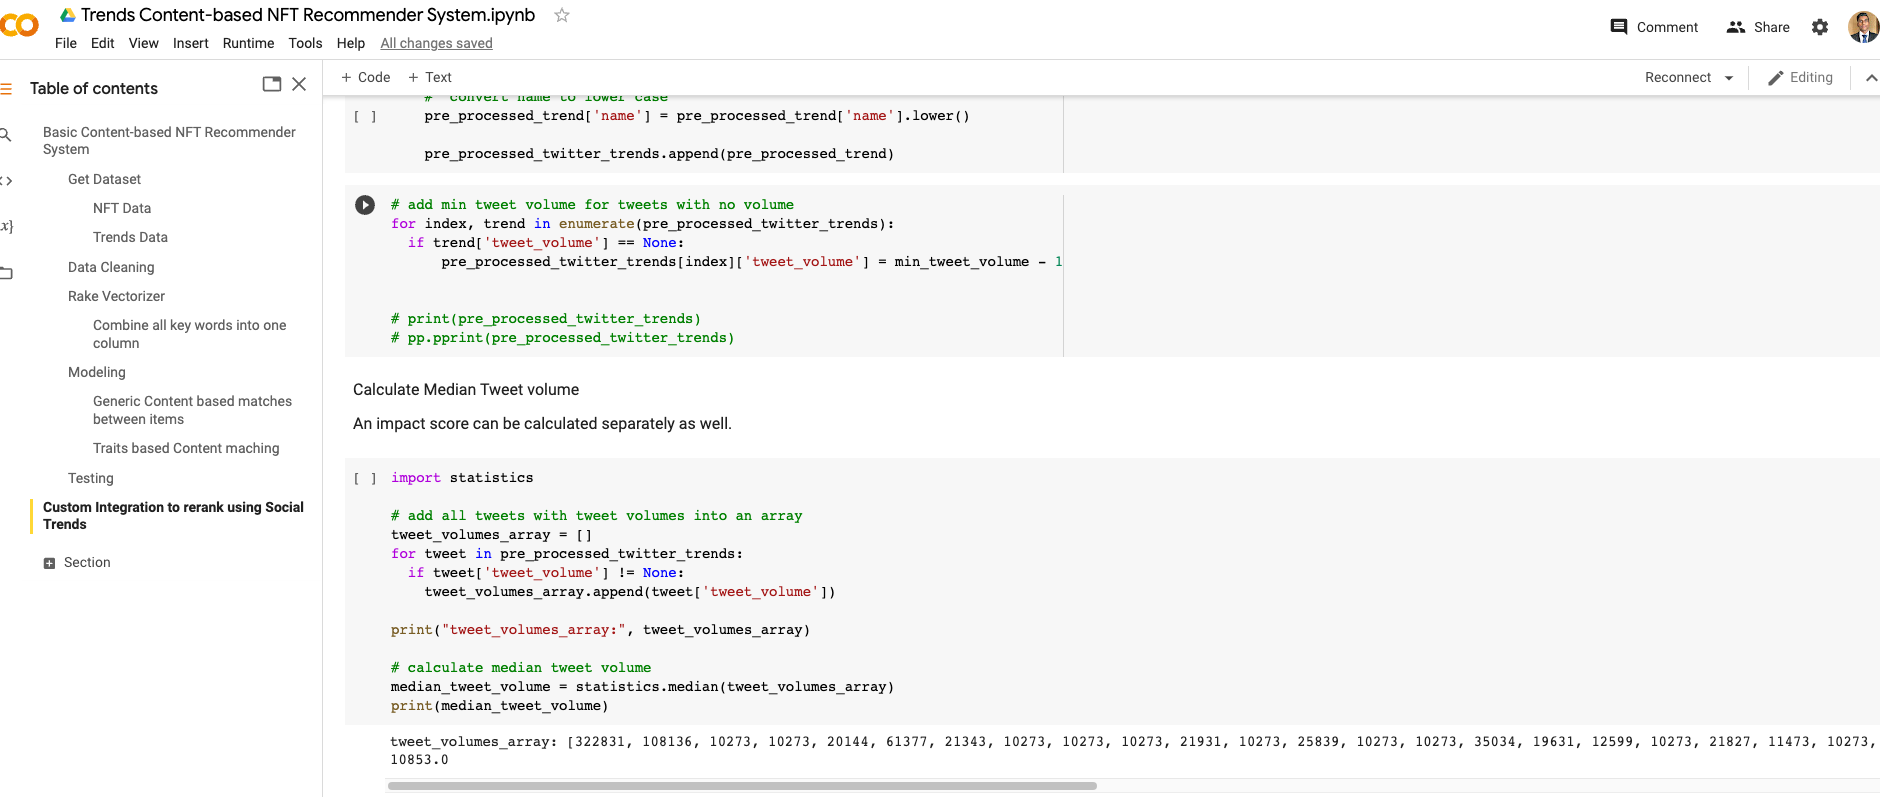
\includegraphics[width=0.95\textwidth]{images/Implementation/code/tweet-volume calculation.png}
\caption{Implementation code segment: Tweet volume calculation \textit{(self-composed)}}
\label{fig:code-tweet-volume-calculation}
\end{figure}

\newpage
\section*{Appendix D2 - UI Wireframes}

\begin{figure}[h!]
\centering
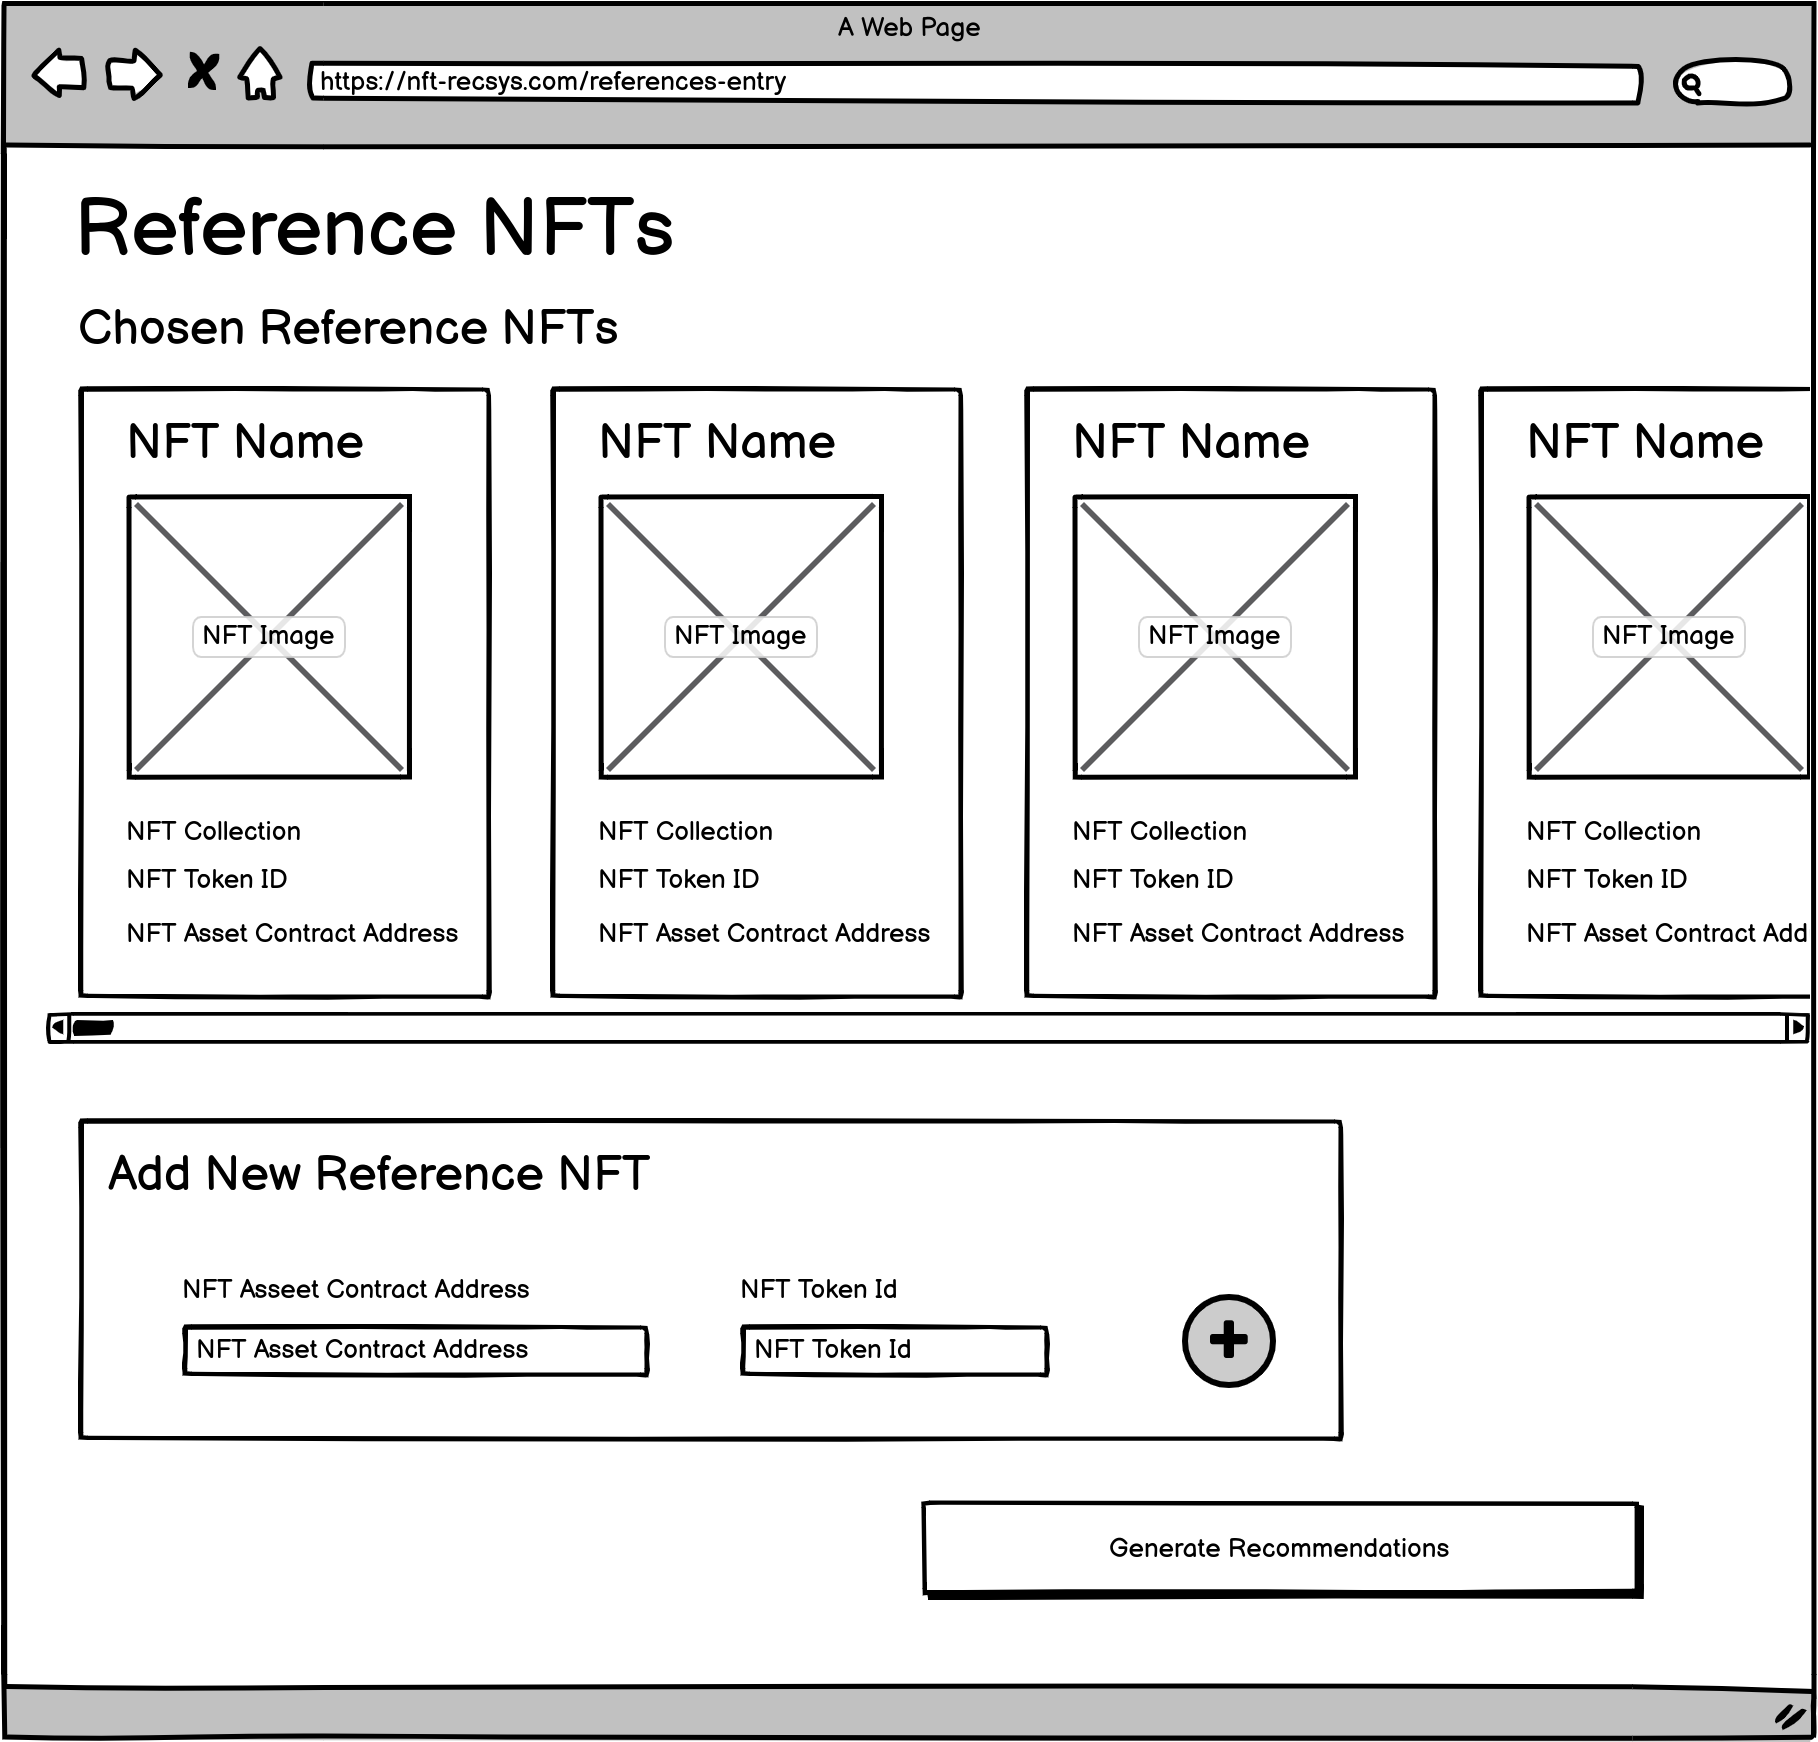
\includegraphics[width=\textwidth]{images/appendix/UI Wireframes/Reference NFT entry.png}
\caption{UI Wireframe - Reference NFT entry \textit{(self-composed)}}
% \label{fig:ui-wireframes-1}
\end{figure}

\begin{figure}[h!]
\centering
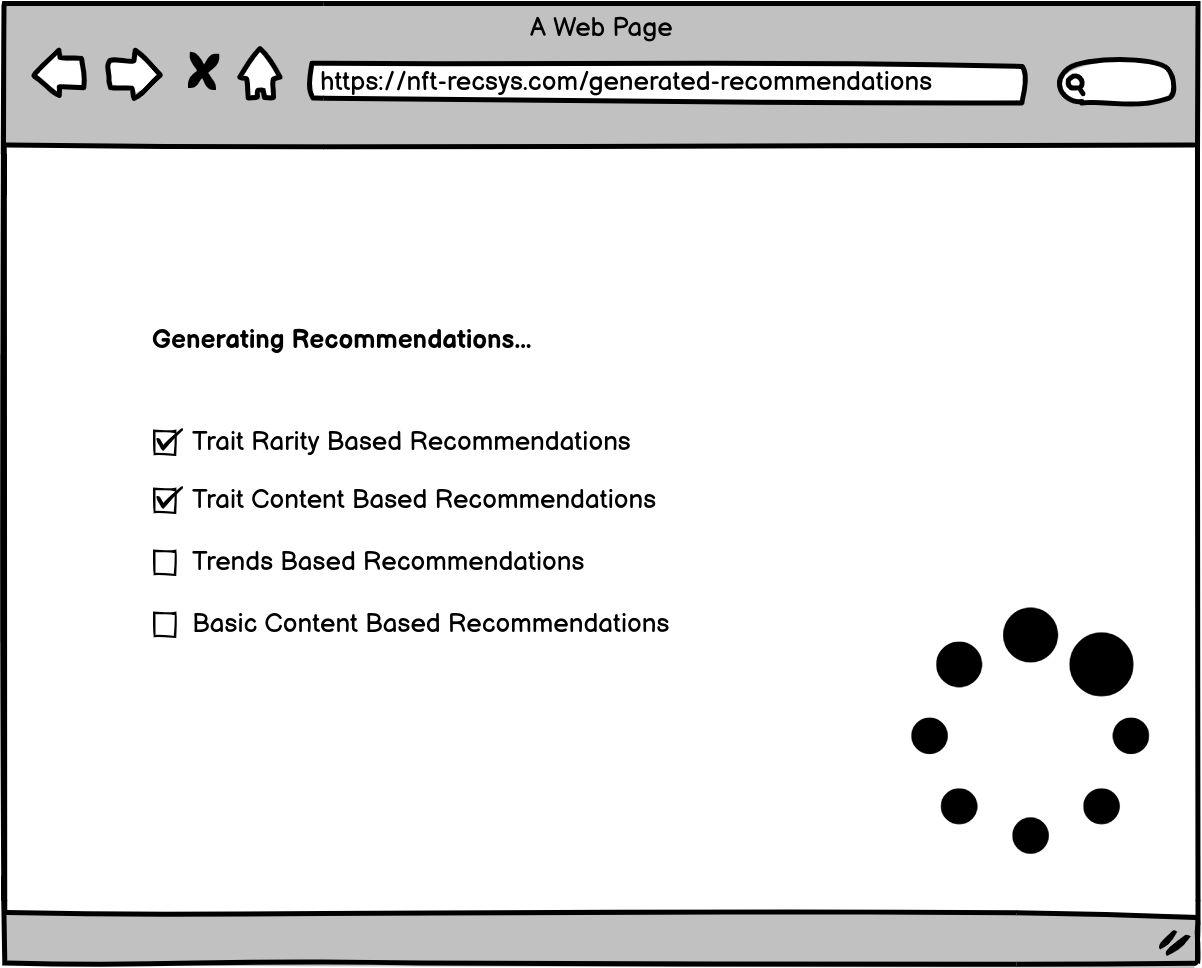
\includegraphics[width=\textwidth]{images/appendix/UI Wireframes/Loading-Generating Recommendations.png}
\caption{UI Wireframe - Loading-Generating Recommendations \textit{(self-composed)}}
% \label{fig:ui-wireframes-1}
\end{figure}

\begin{figure}[h!]
\centering
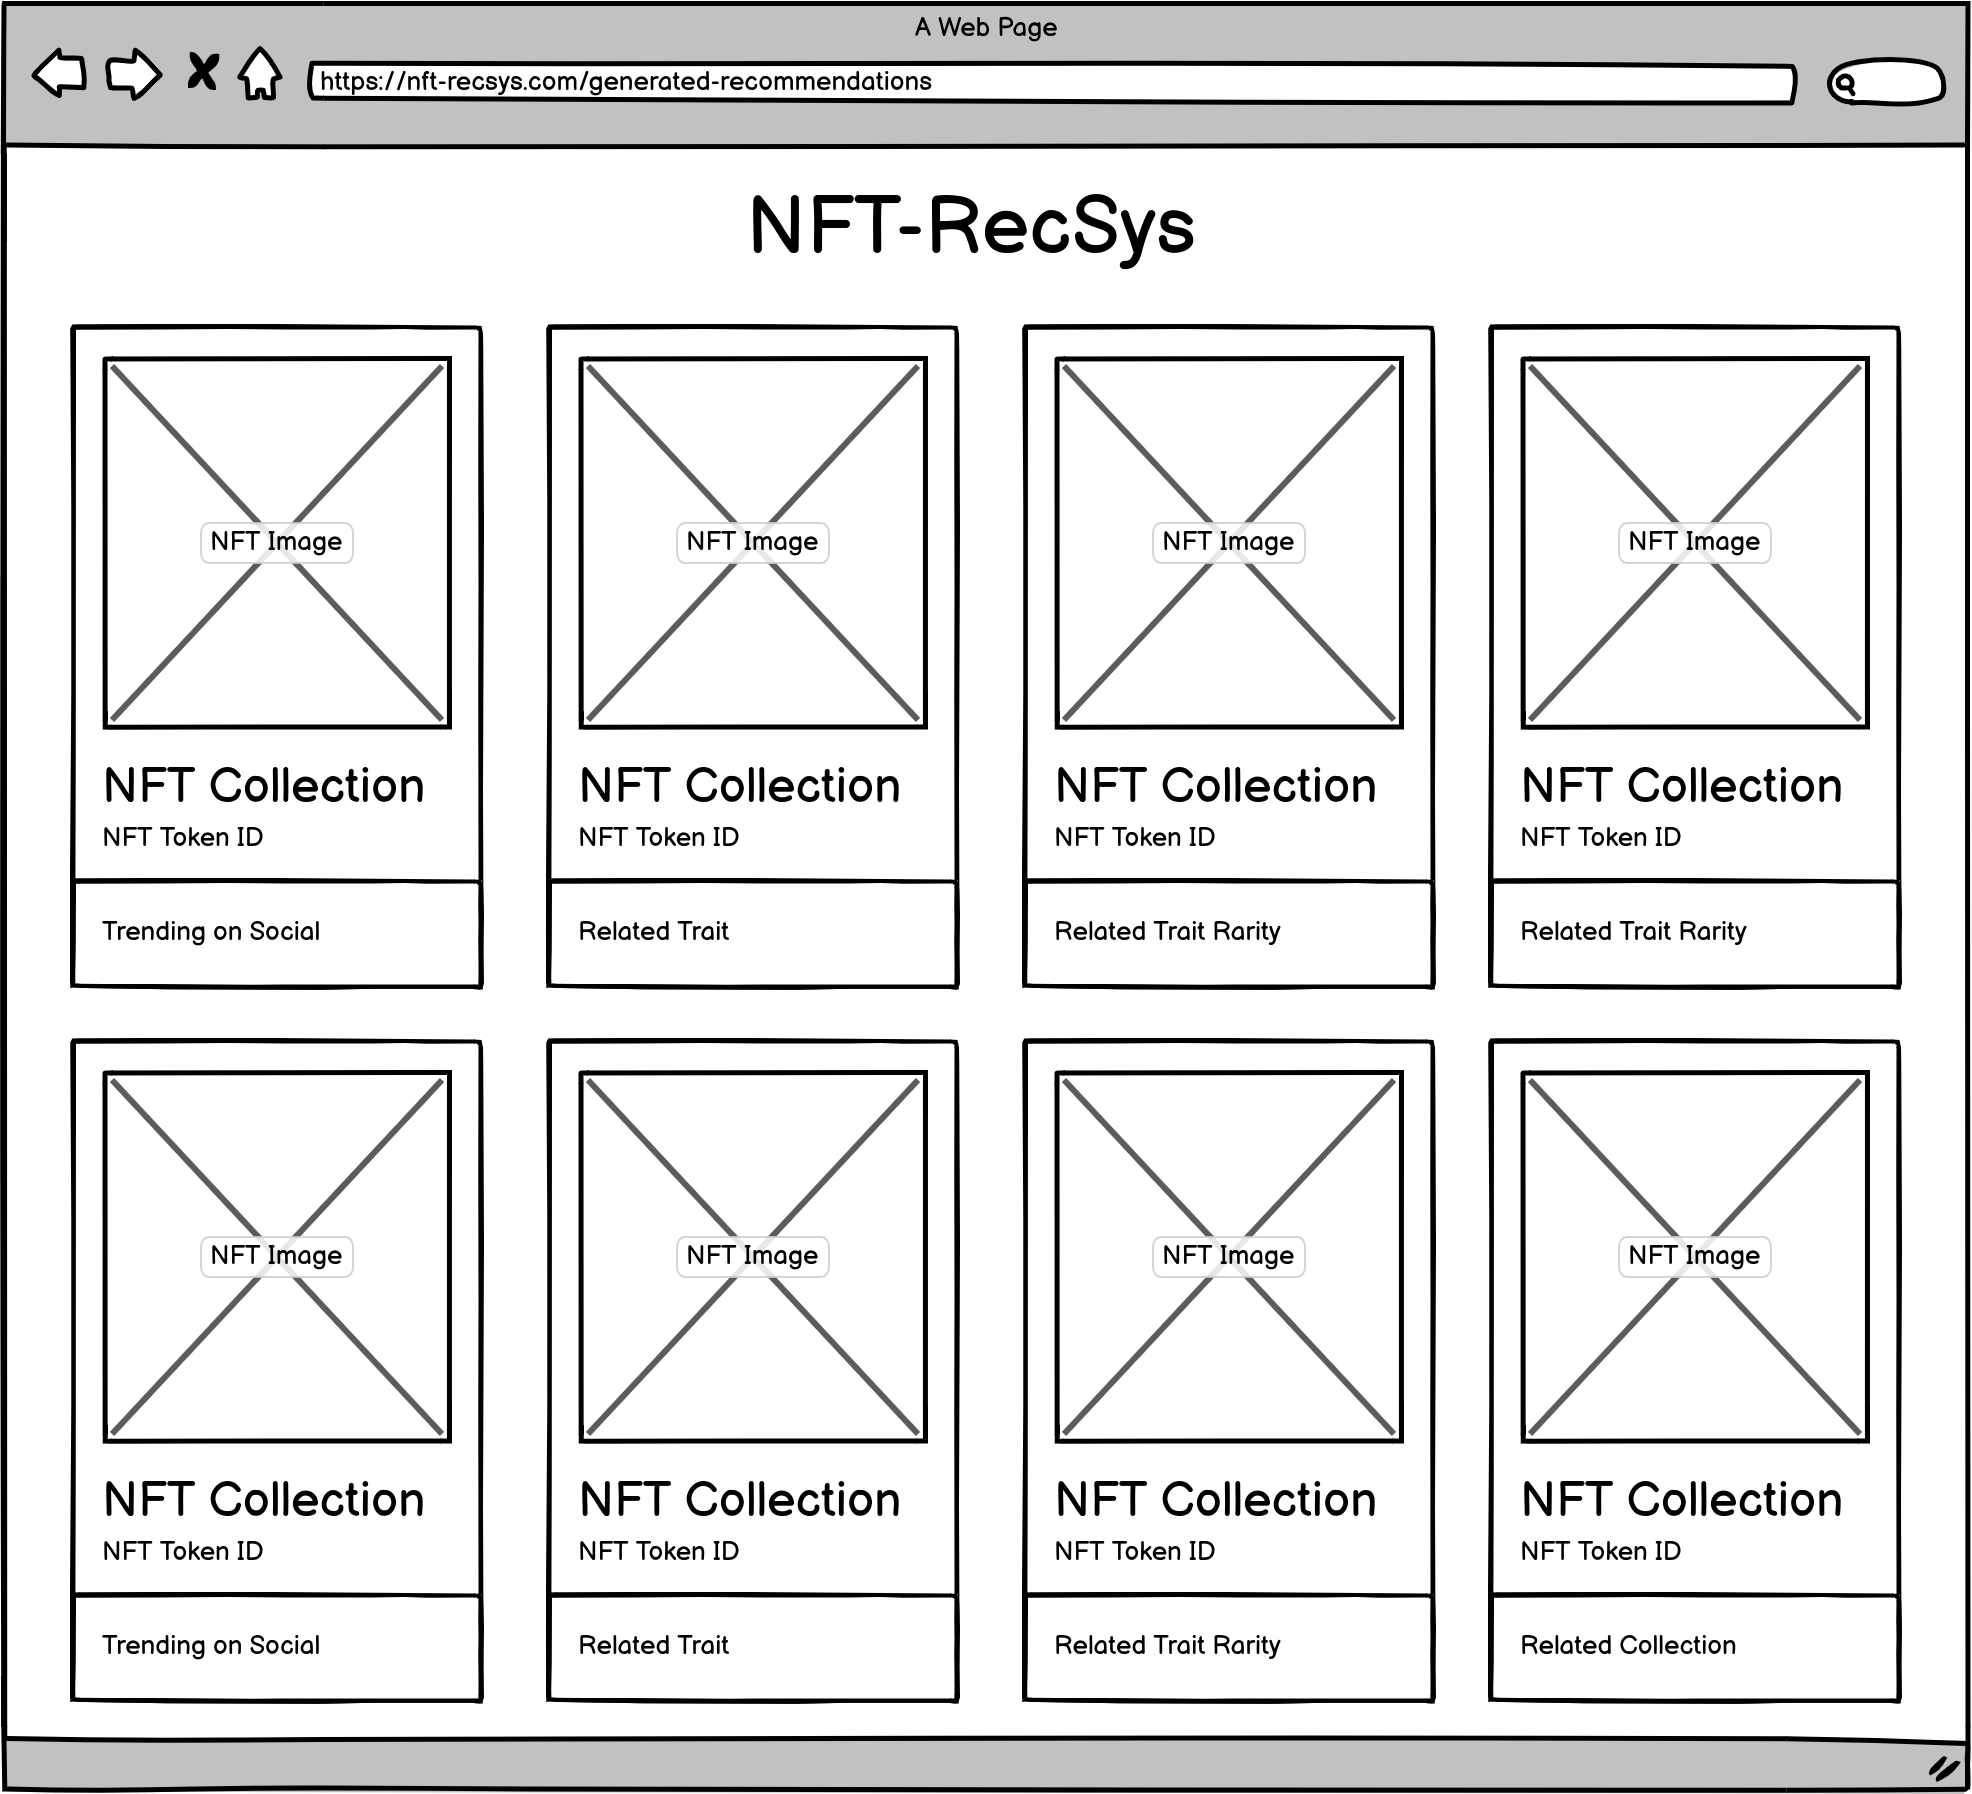
\includegraphics[width=\textwidth]{images/appendix/UI Wireframes/Generated Recommendations.png}
\caption{UI Wireframe - Generated Recommendations \textit{(self-composed)}}
% \label{fig:ui-wireframes-1}
\end{figure}

\begin{figure}[h!]
\centering
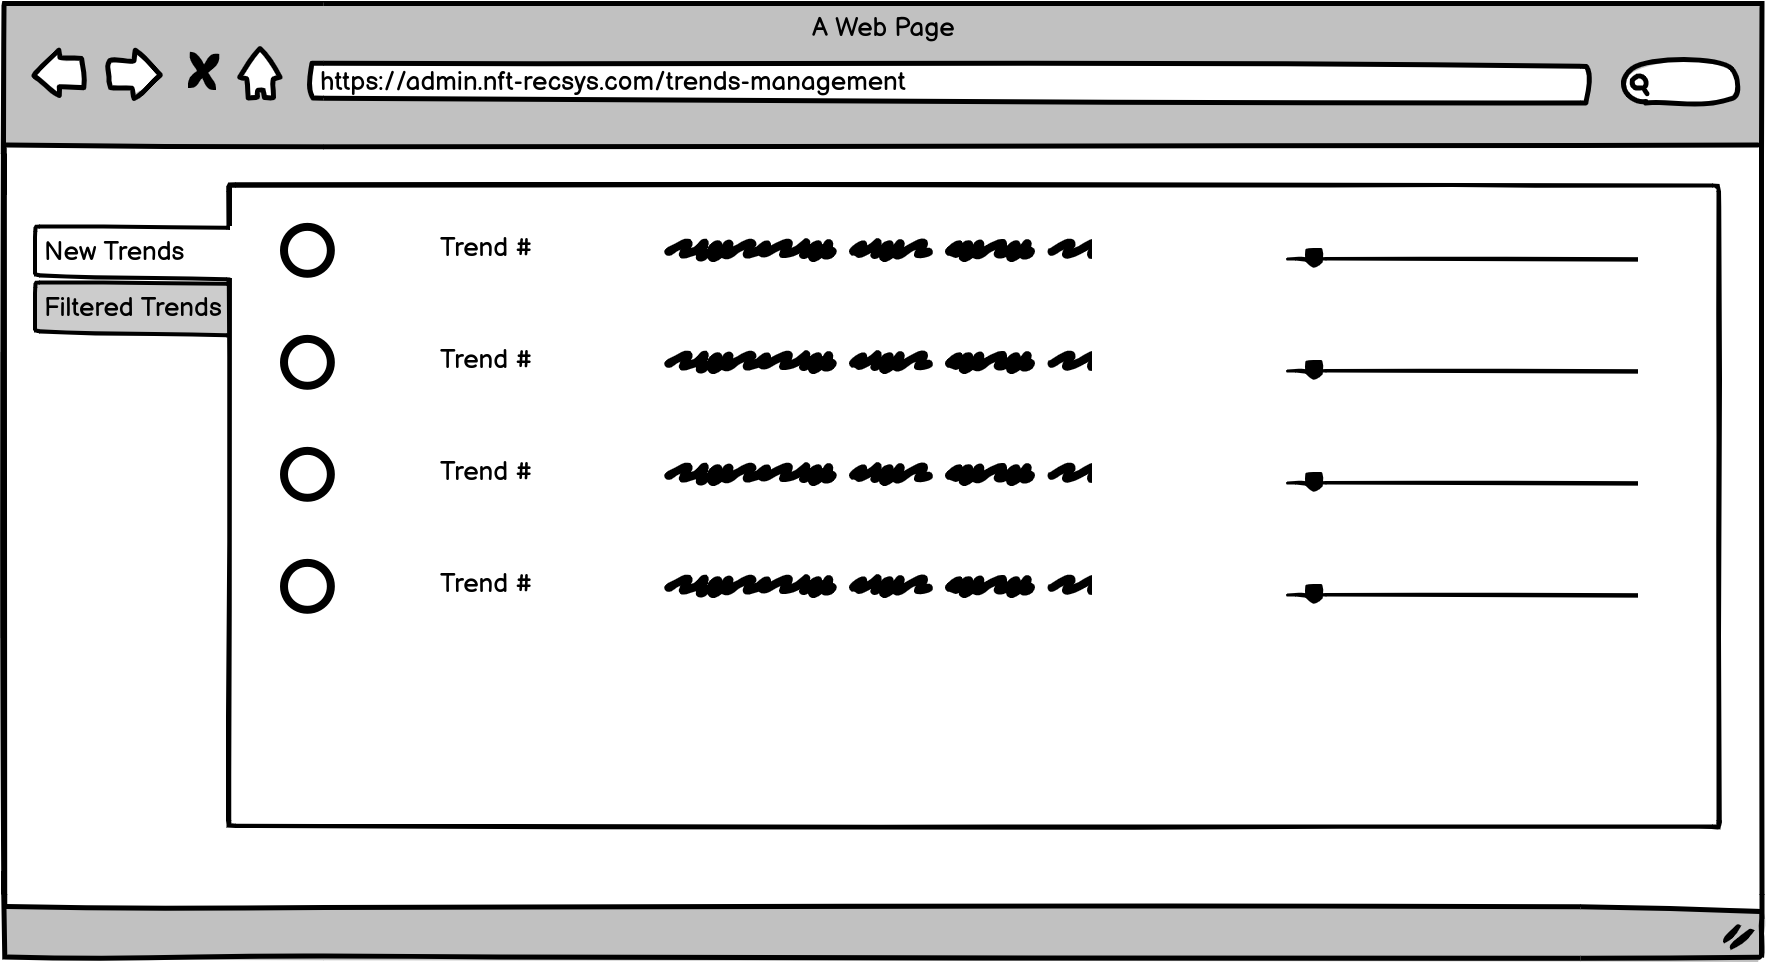
\includegraphics[width=\textwidth]{images/appendix/UI Wireframes/Admin Trends.png}
\caption{UI Wireframe - Admin Trends \textit{(self-composed)}}
% \label{fig:ui-wireframes-1}
\end{figure}

\begin{figure}[h!]
\centering
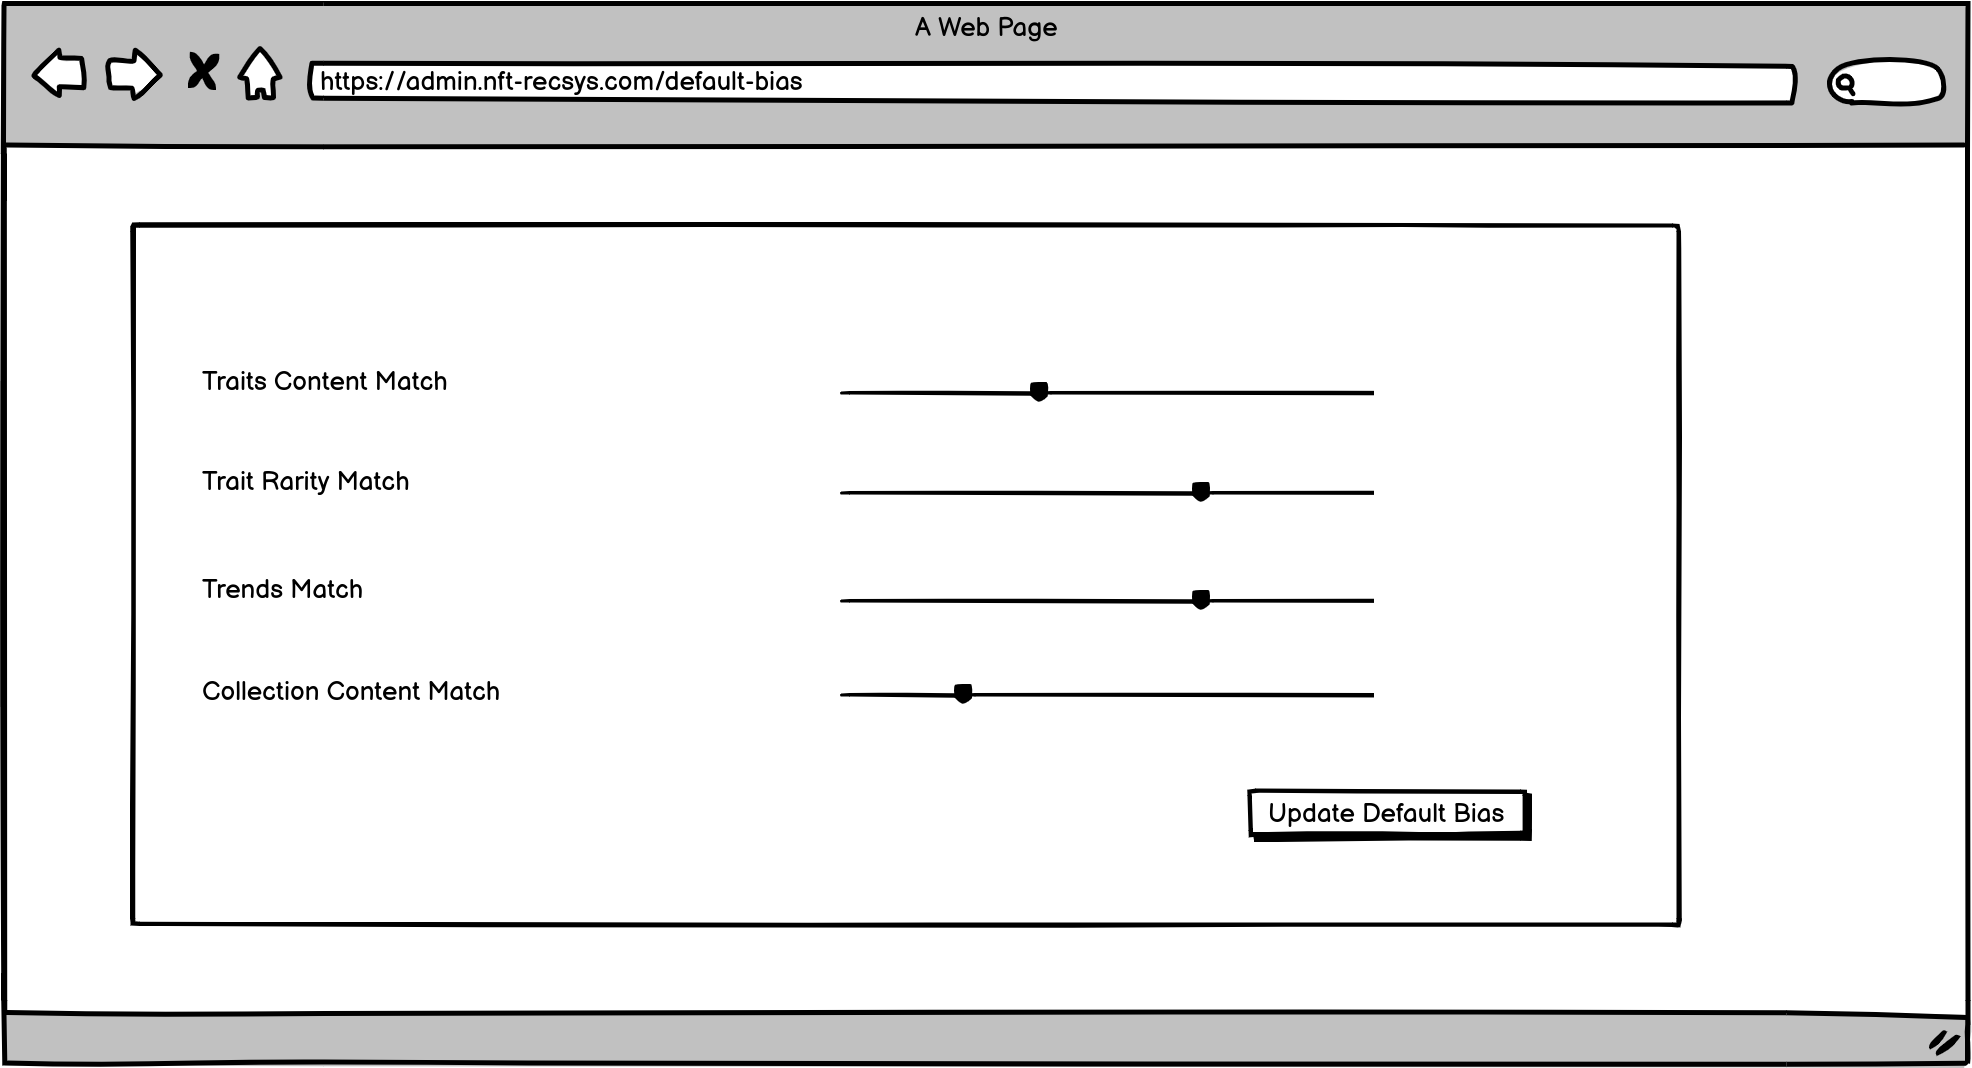
\includegraphics[width=\textwidth]{images/appendix/UI Wireframes/Admin Default Bias selection.png}
\caption{UI Wireframe - Admin Default Bias selection \textit{(self-composed)}}
% \label{fig:ui-wireframes-1}
\end{figure}

\begin{figure}[h!]
\centering
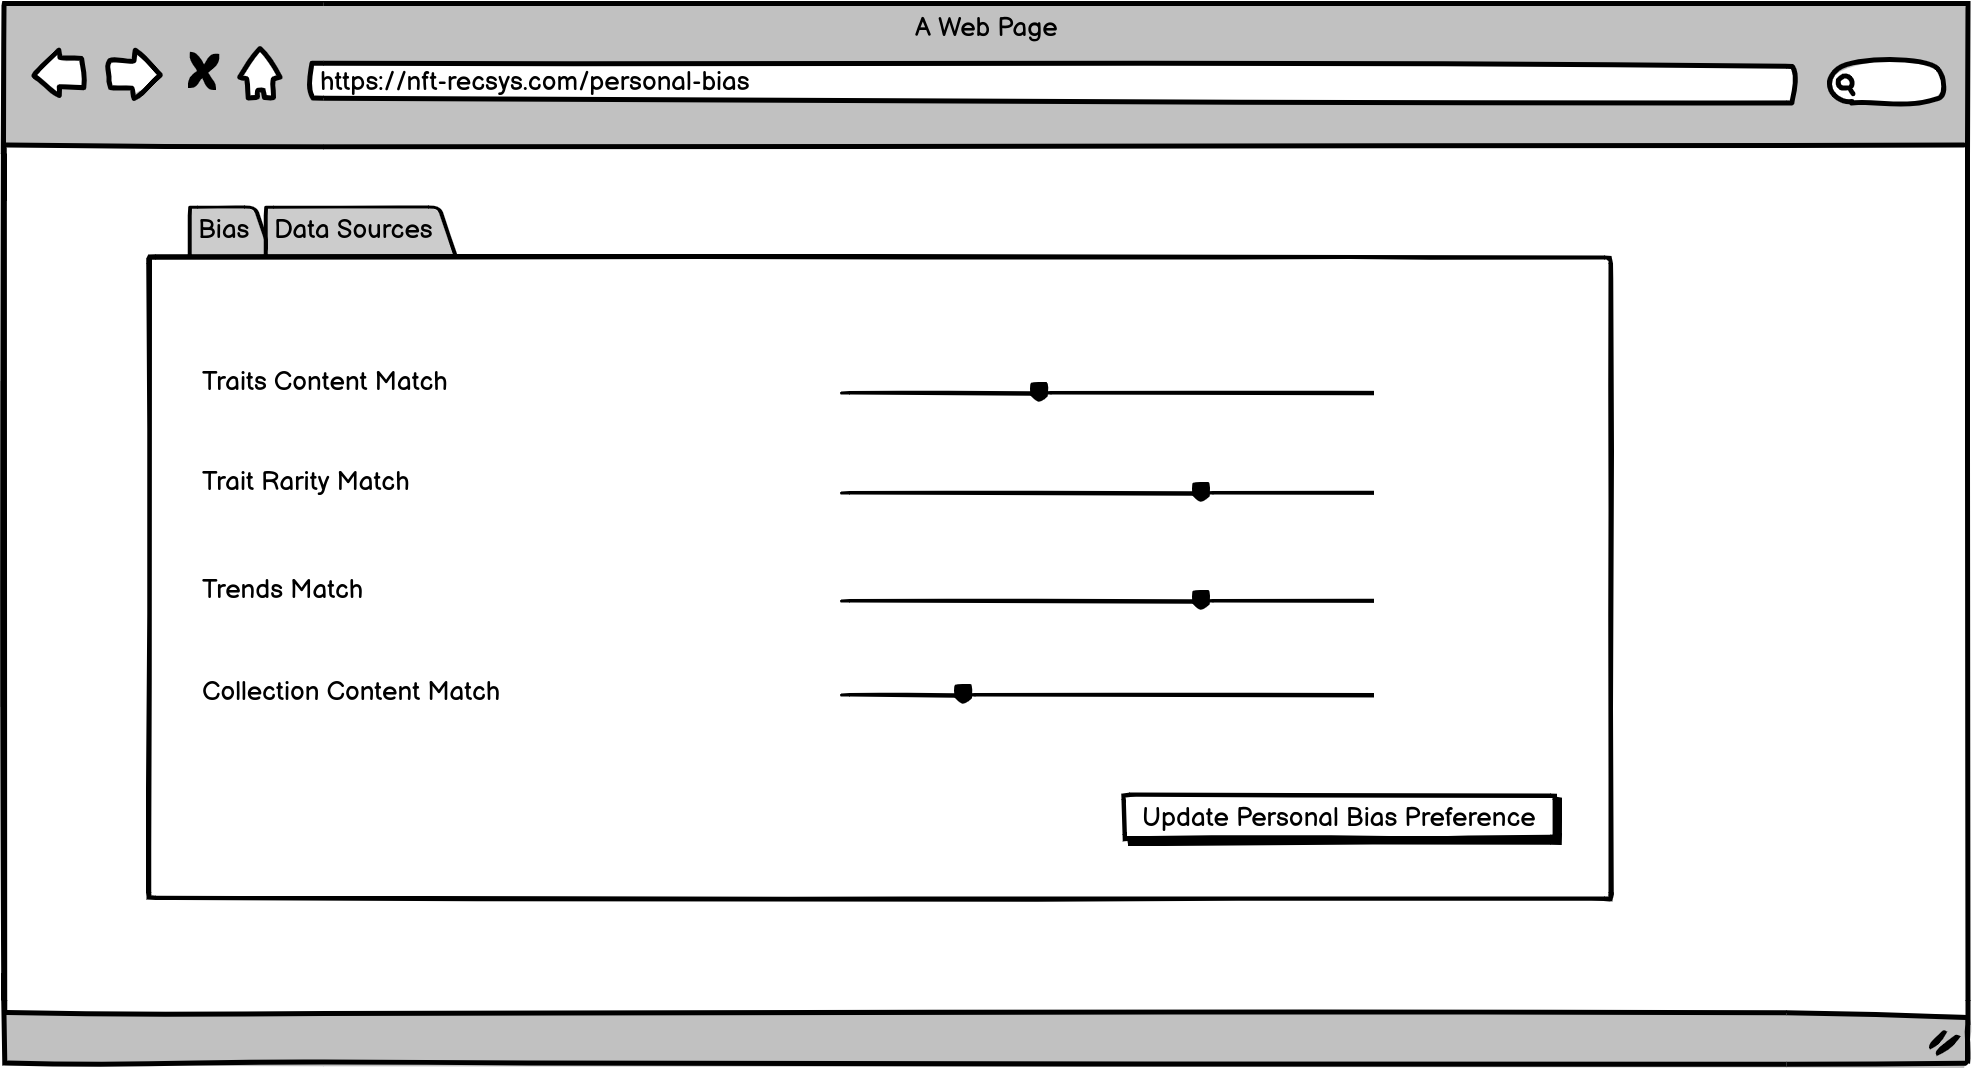
\includegraphics[width=\textwidth]{images/appendix/UI Wireframes/User Bias selection.png}
\caption{UI Wireframe - User Bias selection \textit{(self-composed)}}
% \label{fig:ui-wireframes-1}
\end{figure}


\chapter{Appendix E - Testing}
\label{appendix:testing}

\section*{Appendix E1 - Model Testing}

\begin{figure}[h!]
\centering
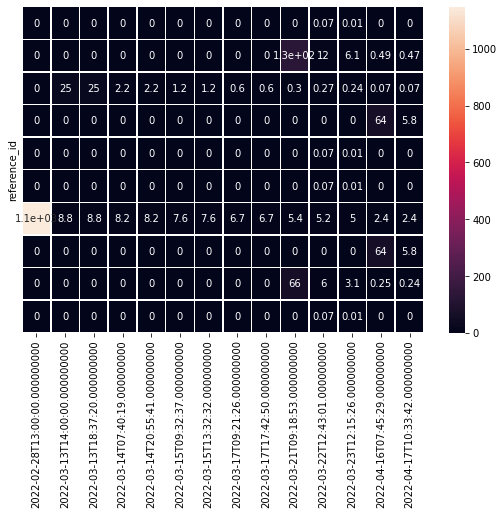
\includegraphics[width=0.6\textwidth]{images/Testing/trends/trends-heatmap-10-rand-annot.png}
\caption{Trends based Recommender Testing Annotated Heatmap - 10 random items \textit{(self-composed)}}
\label{fig:trends-recsys-heatmap-10-anot}
\end{figure}

\begin{figure}[h!]
\centering
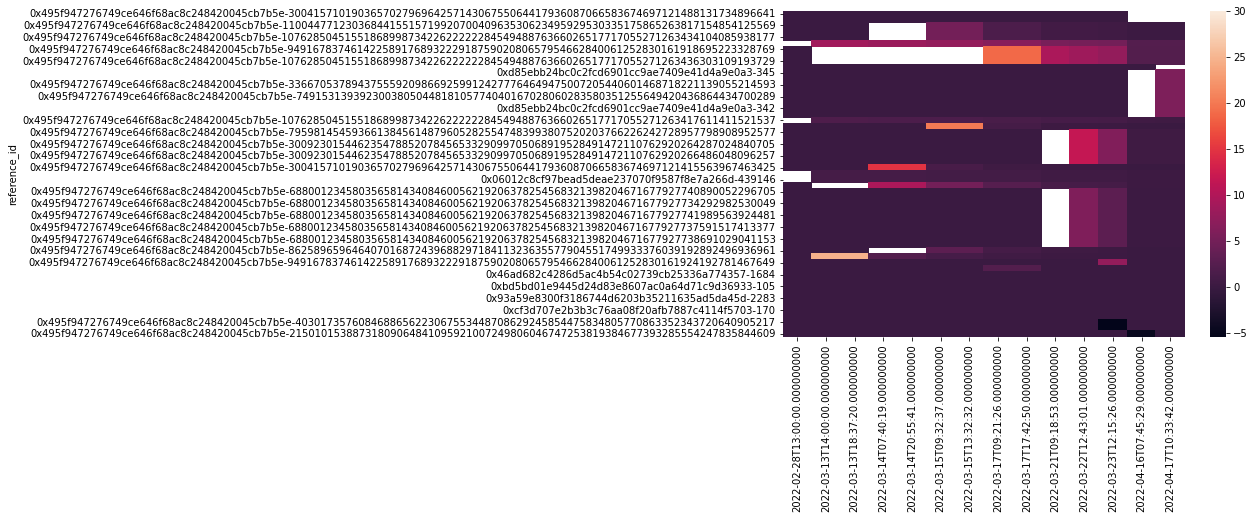
\includegraphics[width=\textwidth]{images/Testing/trends/trends-heatmap-30-labeled.png}
\caption{Trends based Recommender Testing Heatmap - max score 30 \textit{(self-composed)}}
\label{fig:trends-recsys-heatmap-30-labeled}
\end{figure}

\begin{figure}[h!]
\centering
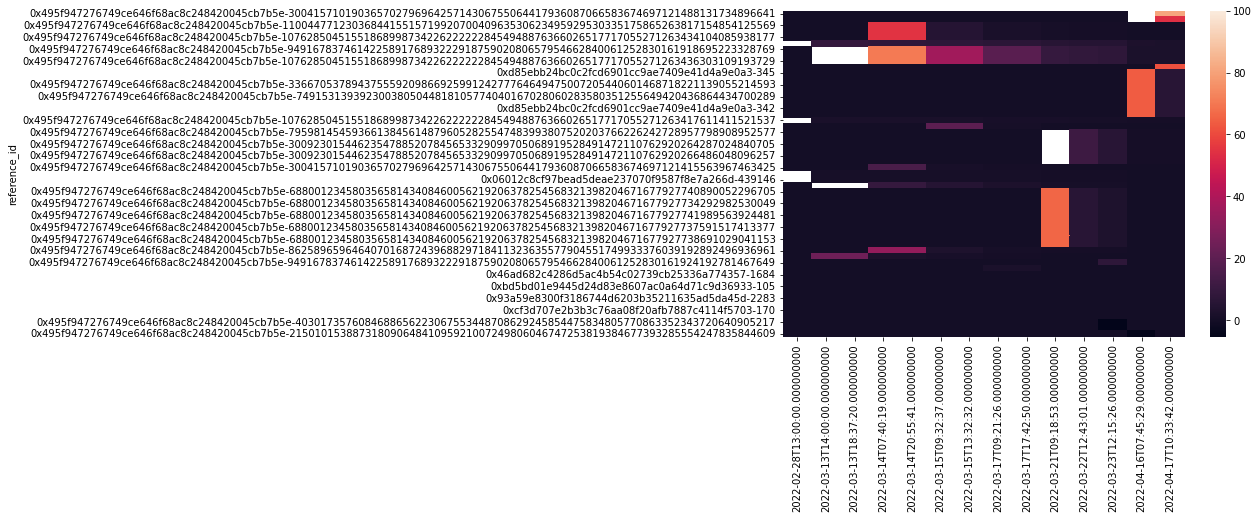
\includegraphics[width=\textwidth]{images/Testing/trends/trends-heatmap-100.png}
\caption{Trends based Recommender Testing Heatmap - max score 100 \textit{(self-composed)}}
\label{fig:trends-recsys-heatmap-100}
\end{figure}

\begin{figure}[h!]
\centering
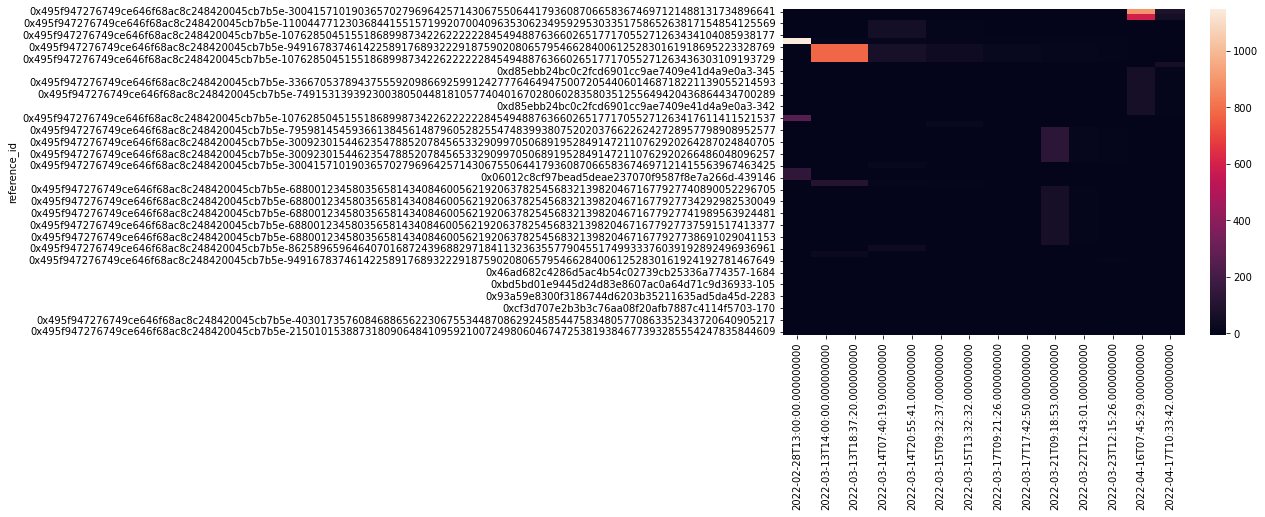
\includegraphics[width=\textwidth]{images/Testing/trends/trends-heatmap-all.png}
\caption{Trends based Recommender Testing Heatmap - All items \textit{(self-composed)}}
\label{fig:trends-recsys-heatmap-all}
\end{figure}

\begin{figure}[h!]
\centering
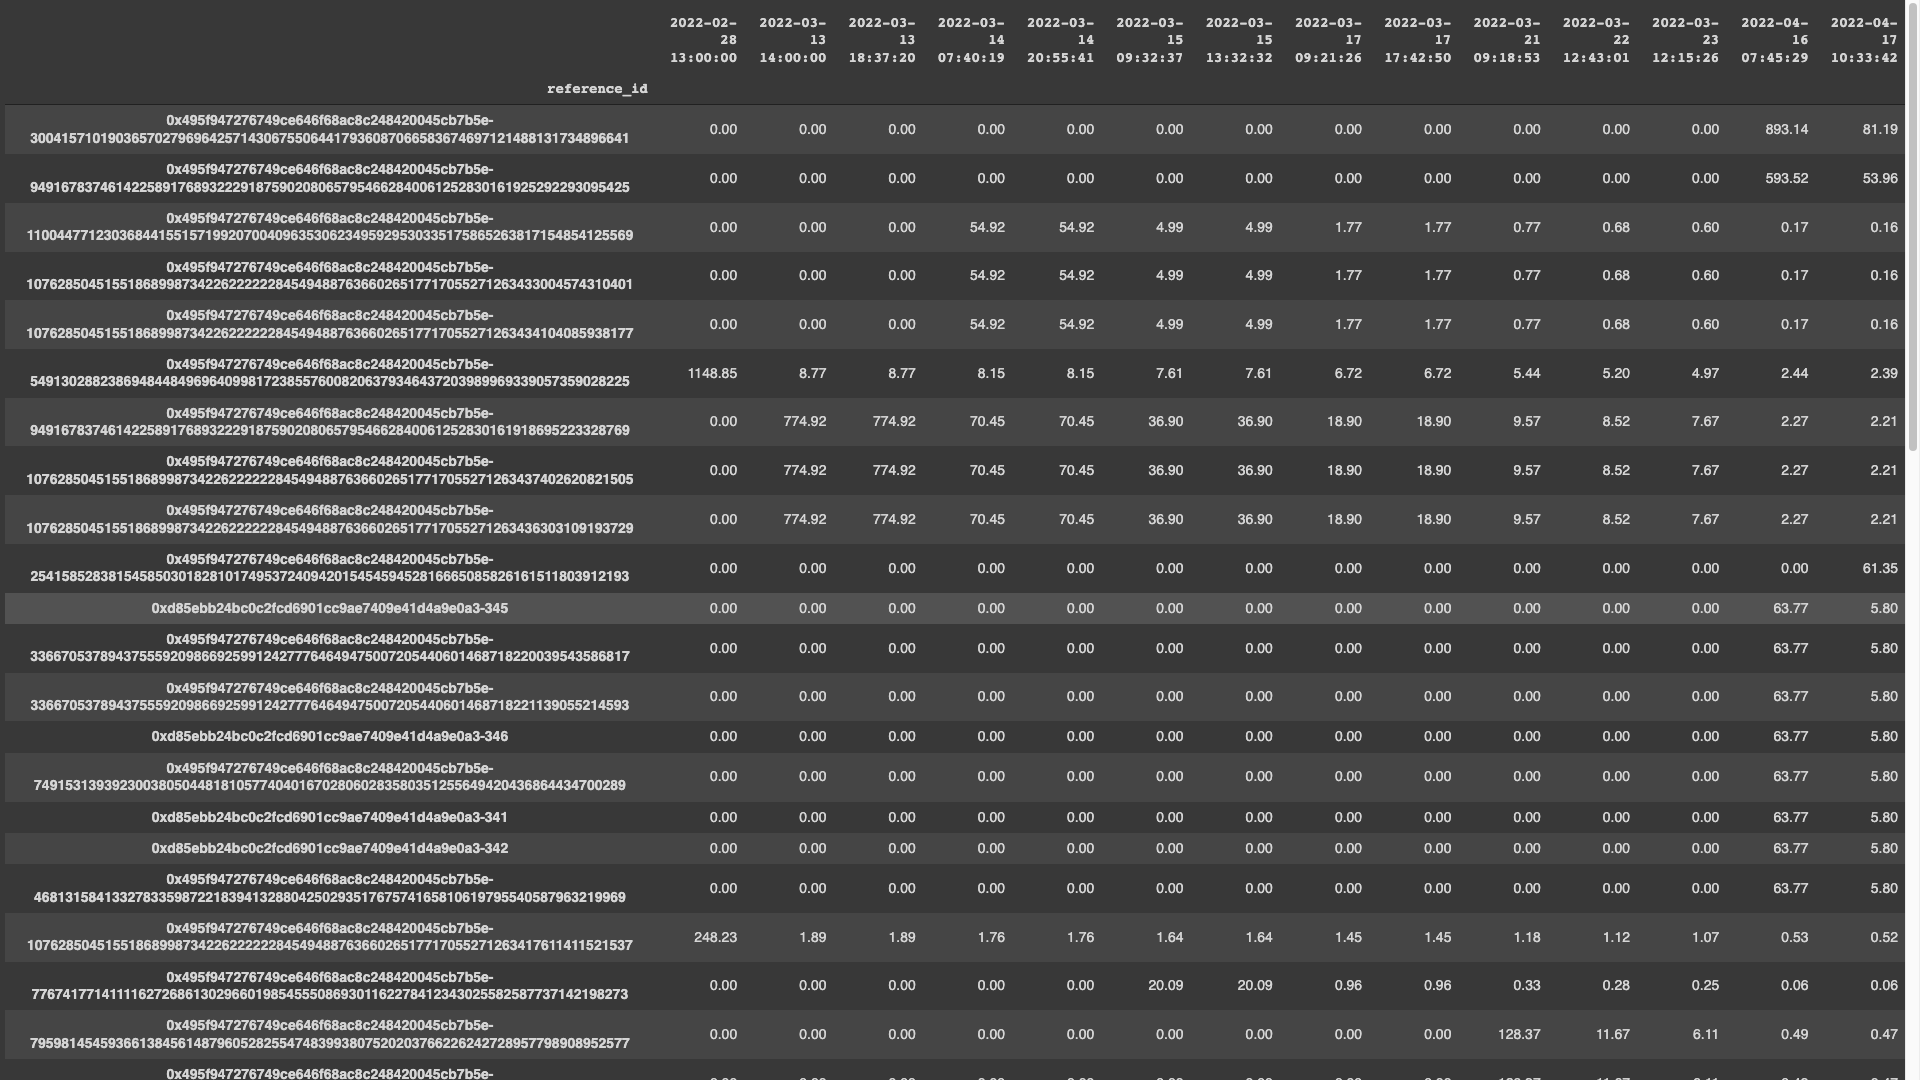
\includegraphics[width=\textwidth]{images/Testing/trends/heatmap-data.png}
\caption{Trends based Recommendations Heatmap Data \textit{(self-composed)}}
\label{fig:trends-recsys-heatmap-data-matrix}
\end{figure}


\clearpage
\section*{Appendix E2 - Model Evaluation of Test Results}

\begin{figure}[h!]
\centering
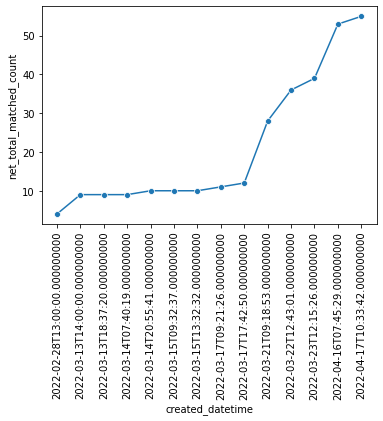
\includegraphics[width=0.6\textwidth]{images/Testing/trends/trends-matches-eval2.png}
\caption{Total Trends based Recommendations made with time \textit{(self-composed)}}
\label{fig:trends-recsys-total-matches}
\end{figure}

\begin{figure}[h!]
\centering
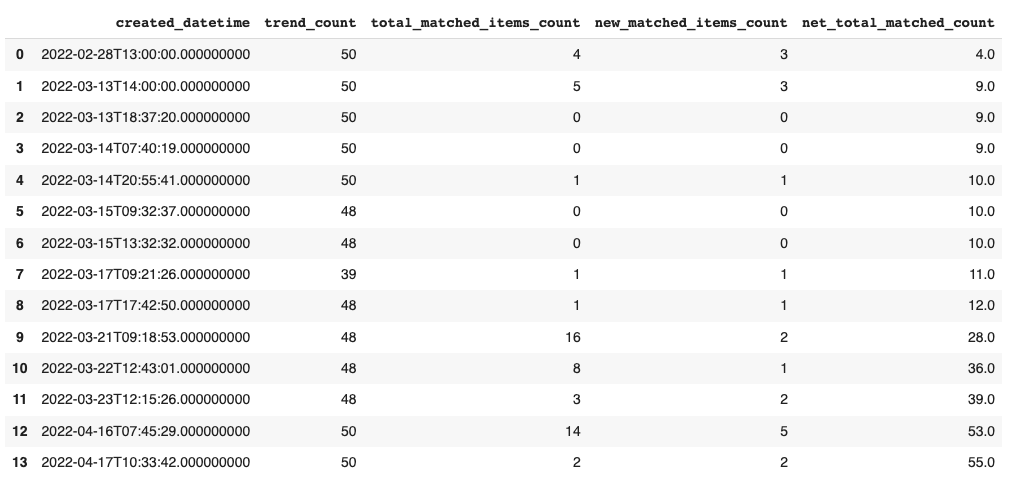
\includegraphics[width=\textwidth]{images/Testing/trends/trend-match-count-data.png}
\caption{Trends based Recommendations Trends Matches Data \textit{(self-composed)}}
\label{fig:trends-recsys-trends-matches-data}
\end{figure}

\begin{figure}[h!]
\centering
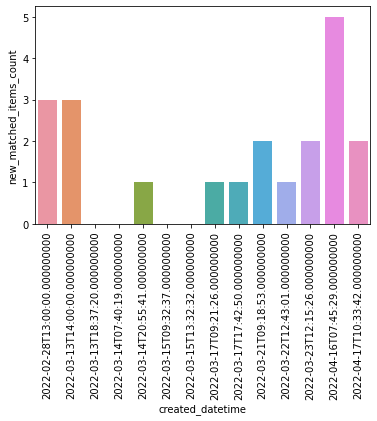
\includegraphics[width=0.6\textwidth]{images/Testing/trends/new_matched_items_per_day.png}
\caption{Trends based Recommendations Newly Matched Items \textit{(self-composed)}}
\label{fig:trends-recsys-trends-new-matches}
\end{figure}

\begin{figure}[h!]
\centering
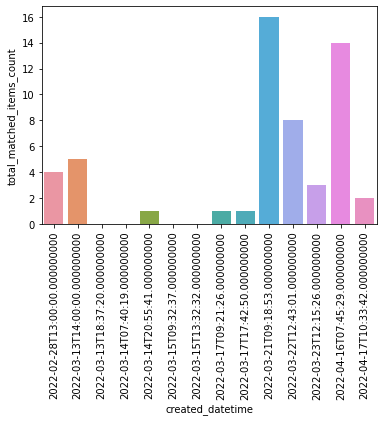
\includegraphics[width=0.6\textwidth]{images/Testing/trends/total_matched_items_per_day.png}
\caption{Trends based Recommendations Total Matched Items \textit{(self-composed)}}
\label{fig:trends-recsys-trends-total-matches}
\end{figure}

\clearpage
\section*{Appendix E3 - Functional Testing}

\vspace{-4mm}
\begin{longtable}{|l|l|p{0.22\linewidth}|p{0.21\linewidth}|p{0.21\linewidth}|l|}
\caption{Testing results of Functional Requirements}
\label{tab:test-func-requirements}
\\ 
\hline
\begin{tabular}[c]{@{}l@{}}\textbf{Test}\\\textbf{Case}\end{tabular}
&
\begin{tabular}[c]{@{}l@{}}\textbf{FR}\\\textbf{ID}\end{tabular}
&
\begin{tabular}[c]{@{}c@{}}\textbf{User}\\\textbf{Action}\end{tabular}
&
\begin{tabular}[c]{@{}c@{}}\textbf{Expected}\\\textbf{Result}\end{tabular} & 
\begin{tabular}[c]{@{}c@{}}\textbf{Actual}\\\textbf{Result}\end{tabular} & \begin{tabular}[c]{@{}c@{}}\textbf{Result}\\\textbf{Status}\end{tabular}
\endfirsthead 
\hline
1 & FR1 & Users adds a chosen \gls{nft} to be considered as the reference & item details are fetched and validated & item details were fetched and validated & Passed \\ 
\hline
2 & FR2 & Admins adds a collection of \gls{nft}s to be used as recommendations. & The details of the \gls{nft}s get fetched and pre-processed for recommendations & The details of the \gls{nft}s were fetched and pre-processed for recommendations & \\ 
\hline
3 & FR3 & A user enters a contract address \& token Id of an \gls{nft}. & The system fetches relevant data of the \gls{nft} & The system fetched relevant data of the \gls{nft} & Passed \\ 
\hline
4 & FR4 & Users sets/ adjusts the bias and parameters to be used & The user specific bias and general bias get adjusted & The user specific bias and general bias were adjusted & \\
\hline
5 & FR5 & Admins adjusts the admin bias & The admin-bias gets adjusted in the system & The admin-bias was adjusted in the system & \\ 
\hline
6 & FR6 & Users clicks a button to generate recommendations & Recommendations are generated and made visible to the user & Recommendations were generated and made visible to the user & Passed \\
\hline
7 & FR7 & A user enters feedback regarding the satisfaction level of the generated recommendations & The feedback of the user is collected and stored in the Database & The feedback of the user was collected and stored in the Database & \\
\hline
8 & FR8 & User requests the reason for recommending the item & Reasons for recommending each item is displayed & Reasons for recommending each item was displayed & Passed \\
\hline
% 9 & FR9 & The system should generate price predictions and consider the results for recommendations. & S & UC5 & \\ 
% \hline
10 & FR10 & User requests featured trending \gls{nft} recommendations & Opinion mining trends data is used to generate \gls{nft} recommendations. & Opinion mining trends data was used to generate \gls{nft} recommendations. & Passed \\
\hline
11 & FR11 & User inputs data-points such as interested public figures, websites to use as opinion mining data for recommendations & The data-points entered are pre-processed and used for trends based recommendations & The data-points entered were pre-processed and used for trends based recommendations & \\ 
\hline
12 & FR12 & Admins inputs data-points such as interested public figures, websites to use as opinion mining data for recommendations. & The data-points entered are pre-processed and used for trends based recommendations & The data-points entered were pre-processed and used for trends based recommendations & \\
\hline
% 13 & FR13 & User-input could be aggregated and used as a reinforcement learning bias for the Recommendations Model. & C & &  \\
% \hline
% 14 & FR14 & The system will not act as a decentralized system. & W & &  \\
% \hline
\end{longtable}

% \section*{Module \& Integration Testing}



\chapter{Appendix F - Evaluations}
\label{appendix:evaluation}

\section*{Appendix F1 - Evaluations received by Evaluators}

Please refer to the categorization in the table \textit{\textbf{\nameref{tab:categories-of-evaluators}}} to understand the Category Ids used to categorize the evaluators.
% TODO: have a table for each cateogry/ separate by category row.
% OR group evaluators - separate using row with category ID?

\vspace{-4mm}
\begin{longtable}{|p{0.27\linewidth}|p{0.655\linewidth}|}
\caption{Evaluations received by Evaluators}
\label{tab:evaluators-eval-feedback}
\\
\hline
\textbf{Evaluator} & \textbf{Feedback} \endfirsthead
\hline
% name & Qualifications/~ Position of Employment 
\textbf{Mr. Sharmilan Somasundaram}

CEO of Niftron - Blockchain as a Service, Certified Blockchain Solution Architect (CBSA), MSc Big Data Analytics

\textit{Category Id(s): 1, 2}
&  
\textit{"Because there's no system like this, it's a good research. The research project is good because gathering data \& domain side is difficult \& new.
The trends based model needs more evaluation. Try synthesizing data to show how recommended items vary across time. Try to show the significance of using the model."}
\\
\hline
\textbf{Mr. Nipuna Senanayake} 

MS Computer Science (USA), Senior Lecturer - IIT

\textit{Category Id(s): 1}
& 
\textit{"The concept of the trends based recommendations system is good. Evaluation of the trends based model is a bit of a concern. Might be possible to evaluate it by web-scraping.
Good amount of work has been done. Keep up the same enthusiasm for research, it will help in the long run, wherever you go."}
 \\
\hline
\textbf{\textit{Anonymous}}

Blockchain Masters Researcher 

\textit{Category Id(s): 1, 2}
& 
\textit{"The research is good, haven't seen \gls{nft} researches that much, although there're quite a lot of Blockchain researches. Will give an A for the project since proper research has been done with the identified research gap.
Price prediction might be possible using art market pricing (if available) since the \gls{nft} market is similar to the market."}
\\
\hline
\textbf{Mr. Aadhil Rushdy}

Senior Data Engineer/Team Lead - Sysco Labs, MSc Computer Science - specialized in Data Science Engineering \& Analytics (University of Moratuwa)

\textit{Category Id(s): 1}
 &
\textit{"This research becomes a novel solution due to the application of multiple recommendation algorithms to recommend a digital object like NFT that has a high willing to pay and fast moving nature. Considering the value of the object with the time and not being sticking to collaborative filtering opens up a good research area. Applying a ensemble of a recommendation approach to mitigate the timely recommendation of objects can be considered as the appropriate approach and the novelty is reflected through this approach. Identifying the research problem followed by identifying technical gaps in recommendation systems is a good starting point to go for the solution. Application of social trends to the recommendation model and the novel trends score calculation algorithm can be considered as a a great contribution by the researcher. Testing and evaluation done on the multiple models and a fair comparison done to show the importance of using both the models.
Could have emphasized on the accuracy of the model since this solution going to impact the end users business or the capital."}
\\
\hline
\textbf{Ms. Areefa Thassim}

Software Engineer - MillenniumIT ESP,
MSc Big Data Analytics

\textit{Category Id(s): 1, 3}
 & 
 \textit{"The research is interesting with NFTs being a relatively new area. The research gap identified is useful for identifying new NFTs. With the NFT marketplace growing rapidly, recommendation systems are going to be needed. The researcher has considered many angles to address the research gap by experimenting with multiple models and approaches. The researcher has excelled in identifying the necessary areas to provide a recommendation to a potential buyer, considering the data that can be accessed for each NFT. The researcher has approached the problem by relating the NFTs as individual products and using their specific traits for recommendation. Since the blockchain is used for privacy and protection of users, this is a good approach. The researcher has provided a good model that has been researched, implemented and evaluated well. A novel approach was provided for recommendations in the NFT domain. The researcher has evaluated the solution well in technical aspects. it would be good if the researcher could approach people and survey them based on the recommendations provided by the recommendation engine. The researcher has evaluated the solution well in technical aspects. it would be good if the researcher could approach people and survey them based on the recommendations provided by the recommendation engine."}
 \\
\hline
\textbf{\textit{Anonymous}}

Data Engineer

\textit{Category Id(s): 1}
&
\textit{"The identified gap seems wide and looks good for an undergraduate research. Recommendation systems and algorithms have been there for a long time now but getting that approach and applying it in a newly rising field such as NFTs is great. The identified wide research gap has been addressed with this research. It is a good approach, implementing multiple types of recommendation models for recommendations based on different aspects. The solution that has been implemented seems to be working fine and the contributions are also great for an undergraduate research. I would suggest to evaluate the implemented models by their performance against some other models in the domain. That would make it easier for anyone to identify where this model stands compared to other models in the domain."}
\\
\hline
\textbf{Mr. Jajeththanan Sabapathipillai}

Chief Product Officer - Niftron, BE (Hons) Computer Software Engineering

\textit{Category Id(s): 2, 3}
 &
 \textit{"Research gap is much needed to analyze the trend as its a NFT hype period and people would love a system to filter the best NFTs to trade. Research has covered the overall area of the research gap. Researcher has approached the research in more generic state where it could have been categorized and analyzed based on several parameters. Valuable NFTs could have evaluated by different parameters such as country, age, domain(art, game NFT), etc. The solution covers recommendations made on top trending NFTs on social media which are most famous ones, but does trending only enough to correlate with the value is the real question here. Should consider NFT utilities, buy and sell trend, no of bids, and visibility as well to identify the top NFTs"}
 \\
\hline
\textbf{Mr. Sasila Hapuarachchi}

 Incoming Engineer - Amazon CA,
 BE Electrical Engineering (Co-op) (Canada)

\textit{Category Id(s): 3}
 & 
 \textit{"The research provides useful background to the topic and the concept map further displays the various sectors of the research. The identified research gap is made clear as NFTs are a relatively new technology and the challenges of NFT recommendation systems can be understood due to their uniqueness. 
 The conducted research discovers areas of exploration to address the research gap by identifying previously researched attempts to address the problem that include content-based, collaborative-based and personalized recommendation systems. The research highlights the potential of matching content with social trends along for better recommendations. 
 The researcher has approached the solution in a comprehensive manner and expands on relevant previous work and ideas. The incorporation of social media throughout the project is also done well.
 The solutions provided in this project take into account a variety of factors that can be useful for the recommendation of NFTs. The use of a trend score in the design is particularly interesting and can be of great benefit to the recommendations as social media has been a major driving force behind the sudden rise in popularity of NFTs. Additionally, incorporating a rarity based model in the design fits well with the overall theme of NFTs and their inherent uniqueness which can drive user interest based on scarcity. Moreover, the content similarity matching model serves as a good integration of existing methodology.
 The developed models were tested and evaluated appropriately. However, it would be useful to see a more comparable evaluation metric for the Trends Based Model to allow for easy comparison with the other models.
 Although specific examples of NFTs are mentioned in the project, it would be useful to see details about the reference NFTs and further clarification on the obtained recommendation results for each model in order to clearly observe their connection to the reference NFT."}
 \\
 \hline
\textbf{Mr. Narada Wickramage}

Assistant Director - MIS \& Statistics, Public Utilities Commission of Sri Lanka, MSc, MBA

\textit{Category Id(s): 3}
& 
 \textit{"NFT market is expected to reach around \$150 billion by 2026 and it is fast growing. NFT trading platforms are available but recommendation systems are not common. Therefore this is a good research area. The research gap has been addressed to a considerable extent. A scientific approach has been taken to approach the solution. Based on tweets but it is sufficient work for an undergraduate project. Evaluation is comprehensive. A suggested improvement is, making this social by developing a social network of participants so that they can collaboratively take part in trading."}
 \\

\hline
% add Achala sir's eval here
\textbf{Mr. Achala Aponso}

Senior Lecturer - IIT, MSc Artificial Intelligence 

\textit{Category Id(s): 1}
 & 
 \textit{"It's a good project overall. What you have discovered is very interesting.
Since only 1 or 2 students in the batch will come up with a new algorithm, the entire focus of the research will be on this.
The selection of parameters have to be confidently explained. Change constants/ parameters and check the output, to show why your selection is correct."}
 \\

% add Prasan sir's eval as well?
\hline
\textbf{Lasal Jayawardena}

% add data science degree stuff...
Undergraduate - BSc (Hons) Artificial Intelligence and Data Science

\textit{Category Id(s): 1, 3}
 & 
 \textit{"It is a interesting research gap that's been addressed here. It is surely the proper direction. The work shown has addressed the research gap. I would say this is a good starting point and will make a good MVP. The solutions \& contributions made have a strong foundation and is well presented. With systems like these you'll need a continuous training system to keep the model up-to-date. I would prefer the testing to be more extensive and have a maybe keep track of ROIs of the recommended NFT to determine performance.
 In a trader's point of view I would prefer trading bots for making quicker trades. In terms of the AI, I feel like the evaluation must be more convincing. And yes its best if you could benchmark the inference speeds of the system just to get a rough idea. 
I think your solutions could be better, if you could direct you focus on artists in particular. Tracking their activity or something along those lines. Reason being I would opt for long term trades where the main factor is the artist rather than the hype. And need to differentiate the model from pump and dumps. Most common pitfall I have seen."}
 \\
\hline
\textbf{Gibran Kasif}

Trainee Software Engineer - Vestoria,
Undergraduate - BSc (Hons) Computer Science

\textit{Category Id(s): 3}
 &
\textit{"This is a new venture especially in the NFT space as this approach has not yet surfaced or ever implemented among major NFT marketplaces such as Opensea, Axie Marketplace and Binance etc. The gap identified is relevant to the concept of a NFT, since an NFT asset is usually sold in limited supply or as a single unit. This is one of the main challenges that come with purchasing an NFT,  to which the following research is expected to resolve. Yes, the conducted research has been able to address the identified research gap. This approach taken isn’t yet noticed on NFT marketplaces, but by introducing such a system would become a versatile tool to the user/consumer interested in purchasing an NFT. 
Using the trend based model in filtering out NFTs, could present a list of viable assets that are close enough to its existing predecessors traits that had been sold out from the collection, which would have the potential to become more valuable. With that in mind, social influence also does have a positive correlation on the success of an NFT collection/brand. For e.g. CryptoPunks.
With the combined use of the trait content and rarity models, both of which are normally included on a NFT, could allow the end user to tailor the results based on their preferences over such features.
Each model's outcome and results were evidently shown on the summarized research.
Since the research currently focuses on the social trends revolving around NFTs. It might be interesting to see in the future whether the system could also prevent fraudulent NFTs from appearing in the results. As most common NFT scams artificially or hack in order to boost  up their social presence of their NFTs, which would affect the end user if encountered."}
 \\
\hline
\textbf{Nazhim Kalam}

Software Engineering Trainee - 99x,
Undergraduate - BSc (Hons) Computer Science

\textit{Category Id(s): 1}
 & 
 \textit{"Since NFTs started getting attention recently, the identified research gap seems new, which is good. Yes, the conducted research has been able to address the identified research gap. I feel like you have done an in depth research with a lot of statistics which I saw from the video attached. The solution seems pretty good and how the scores for negative, neutral and positive is calculated as a part of the solution is very understandable."}
 \\
\hline
\textbf{Ammar Raneez}

Trainee Software Engineer - 99x,
Undergraduate - BSc (Hons) Computer Science

\textit{Category Id(s): 1, 3}
 & 
 \textit{"Clear gap and issue with the traditional collaborative filtering method has been addressed. Yes, the conducted research has been able to address the identified research gap. A straightforward and methodical approach solving each problem at a time, rather than having a direct jump to model construction, especially since this is a novel research topic. The issue of using only a single model to perform recommendations was clear and the approach taken was explained well.  The approach of using the pre-trained twitter model to conduct a sentiment analysis evaluation was well done and the reasoning for doing so was explained well. This technique of evaluation is pretty much best in class."}
 \\
\hline

%  & \\
% \hline
\end{longtable}

\newpage
\section*{Appendix F2 - Evaluation of Functional Requirements}

\vspace{-4mm}
\begin{longtable}{|l|p{0.5\linewidth}|c|l|l|}
\caption{Evaluation of the implementation of Functional Requirements}
\label{tab:eval-func-requirements}
\\ 
\hline
\begin{tabular}[c]{@{}l@{}}\textbf{FR}\\\textbf{ID}\end{tabular}
& \textbf{Requirement} & \begin{tabular}[c]{@{}c@{}}\textbf{Priority}\\\textbf{Level}\end{tabular} & 
\begin{tabular}[c]{@{}c@{}}\textbf{Use}\\\textbf{Case}\end{tabular} & \textbf{Evaluation}
\endfirsthead 
\hline
FR1 & Users must be able to add a chosen NFT to be considered as the reference point to generating recommendations. & M & UC1 & Implemented \\ 
\hline
FR2 & Admins should be able to add a collection of NFT to be used as recommendations. & S & UC1 & \\ 
\hline
FR3 & The system could be able to fetch relevant data of the NFT using an entered token Id. & C & UC1 & Implemented \\ 
\hline
FR4 & Users must be able to set/ adjust the bias and parameters to be used by the Recommendations System using parametric selections prior to generating recommendations. & M & UC2 & \\ 
\hline
FR5 & Admins should be able to adjust the default bias of the Recommendations System. & S & UC3 & \\ 
\hline
FR6 & Users must be able to view recommendations with the click of a button. & M & UC4 & Implemented \\
\hline
FR7 & The prototype could have an option to receive user feedback regarding the satisfaction level of the generated recommendations by the system. & C & UC4 & \\
\hline
FR8 & The system could show the reasons for recommending each item to users. & C & UC4 & Implemented \\
\hline
FR9 & The system should generate price predictions and consider the results for recommendations. & S & UC5 & \\ 
\hline
FR10 & Opinion mining trends data must be used to generate \gls{nft} recommendations. & M & UC7 & Implemented \\
\hline
FR11 & A user could be allowed to feed data-points such as interested public figures, websites to use as opinion mining data for recommendations. & C & UC8 & \\ 
\hline
FR12 & Admins should be able to~feed data-points such as interested public figures, websites to use as opinion mining data for recommendations. & S & UC8 & \\
\hline
FR13 & User-input could be aggregated and used as a reinforcement learning bias for the Recommendations Model. & C & &  \\
\hline
FR14 & The system will not act as a decentralized system. & W & &  \\
\hline
% FR15 search NFTs by tags?
\multicolumn{5}{|c|}{
Functional Requirement Completion Percentage = $\frac{}{14} * 100$ = \%
}\\
\hline
\end{longtable}


\section*{Appendix F3 - Evaluation of Non-Functional Requirements}

\vspace{-4mm}
\begin{longtable}{|l|l|l|l|}
\caption{Evaluation of the implementation of Non-functional requirements}
\label{tab:eval-non-func-requirements}
\\ 
\hline
\textbf{NFR ID} & \textbf{Requirement} & \textbf{Priority Level} &  \textbf{Evaluation} \endfirsthead 
\hline
1 & Performance & Desirable & Implemented \\ 
\hline
2 & Quality of Output & Important & Implemented \\ 
\hline
3 & Security & Desirable & \\ 
\hline
4 & Usability & Important & \\ 
\hline
5 & Scalability & Desirable & \\
\hline
\multicolumn{4}{|c|}{
Non-Functional Requirement Completion Percentage = $\frac{}{5} * 100$ = \%
}\\
\hline
\end{longtable}

\newpage
\section*{Appendix F4 - Self Evaluation}

% screenshot of job requirement posted for Data science role at OpenSea
\begin{figure}[h!]
\centering
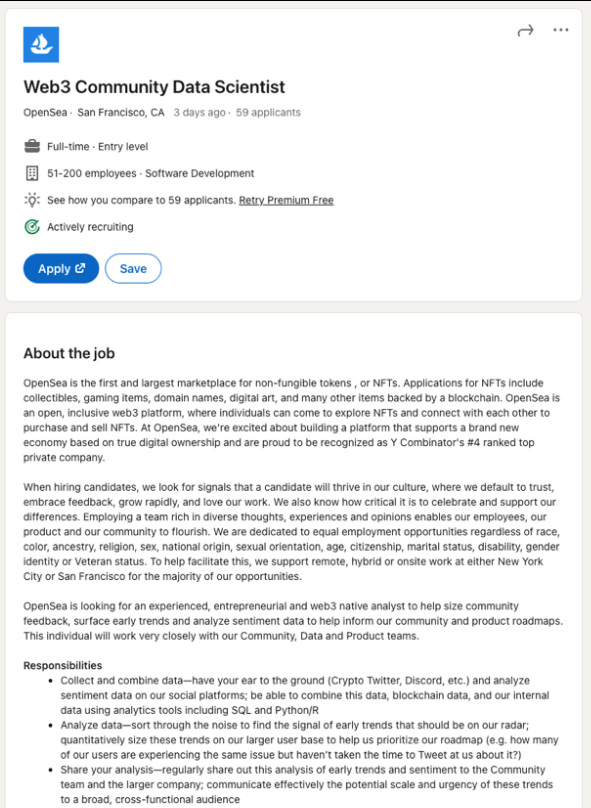
\includegraphics[width=\textwidth]{images/appendix/opensea-datascientist-jobposting.png}
\caption{Screenshot of OpenSea DataScience job posting on LinkedIn - 26/04/2022}
\label{fig:appendix:self-eval}
\end{figure}

\chapter{Appendix G - Conclusion}
\label{appendix:conclusion}

\vspace{-4mm}
\begin{longtable}{| p{0.135\linewidth} | p{0.63\linewidth}| p{0.15\linewidth}|}
\caption{Completion Status of Research Objectives}
\label{tab:research-objectives-status-table}\\
\hline
Objective &  Description & Status \\ 
\hline
% Problem Identification & Identifying a suitable and valuable problem domain to contribute towards, with identified research gaps suitable for a research project.
% & LO5 \\
% \hline
Literature Survey & Read previous work to collate relevant information on related work and critically evaluate them.
\begin{itemize}
\item \textbf{RO1:} Conduct a preliminary study on existing Recommendations Systems \& Architectures.
\item \textbf{RO2:} Analyze the perception of Recommendation techniques.
\item \textbf{RO3:} Conduct a preliminary study on \Gls{nft}s.
\item \textbf{RO4:} Analyze user desires and factors that affect the likability of owning \Gls{nft}s.
\vspace{-7mm}       % remove line spacing after itemize
\end{itemize}
&
Completed\\
\hline
% Project Methodology & Choosing the Research, Development and Project Methodologies that can be followed. Creating a project plan with expected activities and scheduled times for the time frame allocated for the project.
% & LO3, LO7 \\
% \hline
Requirement Analysis &  Specifying the requirements of the project using appropriate techniques and tools in order to meet the expected research gaps \& challenges to be addressed based on previous related research and any domain-specific sources of knowledge.
\begin{itemize}
\item \textbf{RO5:} Gather information about requirements related to desirability of owning \Gls{nft}s \& crypto-related assets.
\item \textbf{RO6:} Gather the requirements of a Recommendations System and understand end-user expectations.
\item \textbf{RO7:} Get insights \&  opinions from technology \& domain experts to build a suitable system.
\vspace{-7mm}       % remove line spacing after itemize
\end{itemize}
&
Completed\\
\hline
Design & Designing architecture and a system that is capable of solving the identified problems with recommended techniques.
\begin{itemize}
\item \textbf{RO8:} Design a price prediction system to identify the possible increase/ decrease in value of the \Gls{nft}s.
\item \textbf{RO9:} Design an automated flow to match \Gls{nft}s with global social trends data.
\item \textbf{RO10:} Design a data-preprocessing pipeline to add Smart Contract data related to \Gls{nft}s in the system.
\item \textbf{RO11:} Design a \Gls{dl} or \Gls{ml} Recommendations model that is capable of appropriately utilizing feature-enhanced data to produce recommendations.
\vspace{-7mm}       % remove line spacing after itemize
\end{itemize}
&
Completed\\
\hline
Development & Implementing a system that is capable of addressing the gaps that were aimed to be solved. 
\begin{itemize}
\item \textbf{RO12:} Develop a Recommendations System that can produce relevant, timely \& trending NFTs (items).
\item \textbf{RO13:} Integrate automation steps in the prototype to enhance features of NFT records and use them to recommend suitable NFTs.
\item \textbf{RO14:} Develop an algorithm that can utilize factors that are considered to affect the desirability of owning an NFT by a person.
\vspace{-7mm}       % remove line spacing after itemize
\end{itemize}
&
Completed\\
\hline
Testing and Evaluation & Testing the created system \& Data science models with appropriate data and evaluating them with baseline techniques identified in the literature. 
\begin{itemize}
\item \textbf{RO15:} Create a test plan and perform unit, integration and functional testing.
\item \textbf{RO16:} Evaluate the novel model by bench-marking with  \Gls{p@k} score, compared against baseline models.
\vspace{-7mm}       % remove line spacing after itemize
\end{itemize}
&
Completed\\
\hline
Documenting the progress of the research & Documenting and notifying the continuous progress of the research project and any faced obstacles. 
&
Completed\\
\hline
Publish Findings & Produce well-structured documentation/ reports/ papers that critically evaluate the research.
\begin{itemize}
\item \textbf{RO17:} Publishing a review paper on related work.
\item \textbf{RO18:} Publishing evaluation \& testing results identified from the research.
\item \textbf{RO19:} Making the code or models created in the research process available for future advancements in research.
\item \textbf{RO20:} Making any modified data-sets or re-creation strategies available to the public, to train \& test models related to similar use cases of utilized data.
\vspace{-7mm}       % remove line spacing after itemize
\end{itemize}
&
Completed\\
\hline
\end{longtable}


% \vspace{-4mm}
\begin{longtable}{|p{0.8\linewidth}|p{0.1471\linewidth}|}
\caption{Achievement of Learning Outcomes}
\label{tab:achievement-learning-outcomes-table}
\\ 
\hline
\textbf{Learnings} & \textbf{LOs}\endfirsthead 
\hline
The identified problem was tackled after selecting \& applying appropriate methods with justifications. & LO1 \\
\hline
Requirements of the project were gathered from literature, surveys \& interviews. Then, the collected requirements were analyzed and clearly indentified. & LO2 \\
\hline
Over 50 literature were read, surveyed, then critically reviewed. & LO4 \\
\hline
There were many tasks that the author had defined and was expected to carry out throughout the research. These tasks were carried out after analyzing all the possible available options. & LO5, LO3 \\
\hline
The supervisor was regularly met and the deliverables were produced as agreed based on a developed project plan that scheduled the required activities to be carried out. & LO6, LO3 \\
\hline
SLEP Issues related to the research were taken note of and mitigated by identifying possible issues and planning ahead of handling those issues. & LO7 \\
\hline
The entire research was documented at the best possible standard \& structure with critical evaluations, following the guidance given by the module leader \& supervisor. The documents included the project proposal, Project Specification \& Prototype Document (PSPD), this thesis, 2 research papers \& 1 review paper. All the papers were published as pre-prints on ArXiv and the research papers were submitted to research conferences. & LO8 \\
\hline
\end{longtable}